\documentclass[openany]{book}
\author{David Gabriel Corzo Mcmath}
\title{Matemática Discreta Aplicada \\ \normalsize Notas de clase}
\date{2019-08-03 02:29}
% % % % % % % % % % % % % % % % % % % % % % % % % % % % % % % % % % % % % % % % % % % % % % % % % % %
\usepackage[margin = 1in]{geometry}
\usepackage{graphicx}
\usepackage{fontenc}
\usepackage{pdfpages}
\usepackage[spanish]{babel}
\usepackage{amsmath}
\usepackage{amsthm}
\usepackage[utf8]{inputenc}
\usepackage{enumitem}
\usepackage{mathtools}
\usepackage{import}
\usepackage{xifthen}
\usepackage{pdfpages}
\usepackage{transparent}
\usepackage{color}
\usepackage{fancyhdr}
\usepackage{lipsum}
\usepackage{sectsty}
\usepackage{titlesec}
\usepackage{calc}
\usepackage{lmodern}
\usepackage{xpatch}
\usepackage{blindtext}
\usepackage{bookmark}

%%%%%%%%%%%%%%%%%%%%%%%%%%%%%%%%%%%%%%%%%%%%%%%%%%%%%%%%%%%%%%%%%%%%%%%%%%%%%%%%%%%%%%%%%%%%%%%%
% Clear the header and footer
\fancyhead{}
\fancyfoot{}
% Set the right side of the footer to be the page number
{\fontfamily{mc}\selectfont
\fancyfoot[L]{\thepage}
\fancypagestyle{plain}{
    \renewcommand{\headrulewidth}{0pt}
    \fancyhf{}
    \fancyfoot[L]{\thepage}
}}

% THIS IS TO CENTER AND DEDICATE A CHAPTER NAME AN ENTIRE PAGE
\titleformat{\chapter}[display]
{\vfill\filcenter}
{{%
   \filcenter\fontsize{48pt}{48pt}\usefont{T1}{cm}{m}{n}{\centering\chaptername} 
   \fontsize{80pt}{80pt}\selectfont\thechapter%
 }%
}
{5pt}
{\huge\usefont{T1}{cm}{b}{n}
 \parbox{\textwidth-\widthof{\LARGE\sffamily{\centering\chaptername}}}
}[\vfill\clearpage]

\titlespacing*{\chapter}{0pt}{0pt}{50pt}

% TO SEPATE WHOLE PAGE DEDICATION IN THE TABLE OF CONTENTS
\titleformat{name=\chapter,numberless}[display]
{\filcenter}
{{
 }
}
{5pt}
{\Huge\usefont{T1}{cm}{b}{n}\centering
}







% MAKE THE TITLE OF THE CHAPTER CENTER!!
\makeatletter

\xpatchcmd{\@makeschapterhead}{%
  \Huge \bfseries  #1\par\nobreak%
}{%
  \Huge \bfseries\centering #1\par\nobreak%
}{\typeout{Patched makeschapterhead}}{\typeout{patching of @makeschapterhead failed}}


\xpatchcmd{\@makechapterhead}{%
  \huge\bfseries \@chapapp\space \thechapter
}{%
  \huge\bfseries\centering \@chapapp\space \thechapter
}{\typeout{Patched @makechapterhead}}{\typeout{Patching of @makechapterhead failed}}

\makeatother

% \newcommand*\circled[1]{\tikz[baseline=(char.base)]{
%             \node[shape=circle,fill=gray!50,inner sep=2pt] (char) {#1};}}

% % header style
% \pagestyle{fancy}
% \fancyhf{}
% \fancyhead[EL]{\nouppercase\leftmark}
% \fancyhead[OR]{\nouppercase\rightmark}
% \fancyfoot[C]{\circled{\thepage}}
\newcommand*\circled[1]{\tikz[baseline=(char.base)]{
            \node[shape=circle,fill=gray!50,inner sep=2pt] (char) {#1};}}

% header style
\pagestyle{fancy}
\fancyhf{}
\fancyhead[EL]{\nouppercase\leftmark}
\fancyhead[OR]{\nouppercase\rightmark}
\fancyfoot[C]{\circled{\thepage}}

\fancypagestyle{plain}{%
  \fancyhf{}
  \fancyfoot[C]{\circled{\thepage}}
  \renewcommand{\headrulewidth}{0pt}
}



% % % % % % % % % % % % % % % % % % % % % % % % % % % % % % % % % % % % % % % % % % % % % % % % % % %
\begin{document}
\maketitle
\tableofcontents

%%%%%%%%%%%%%%%%%%%%%%%%%%%%%%%%%%%%%%%%%%%%%%%%%%%%%%%%%%%%%%%%%%%%%%%%%%%%%%%%%%%%%%%%%%%%%%%%

\part{Notas de Clases del semestre}
\chapter{Clase del Día: 2019-07-22; clase introductoria, ¿qué es la matemática discreta?, juegos de lógica fáciles}
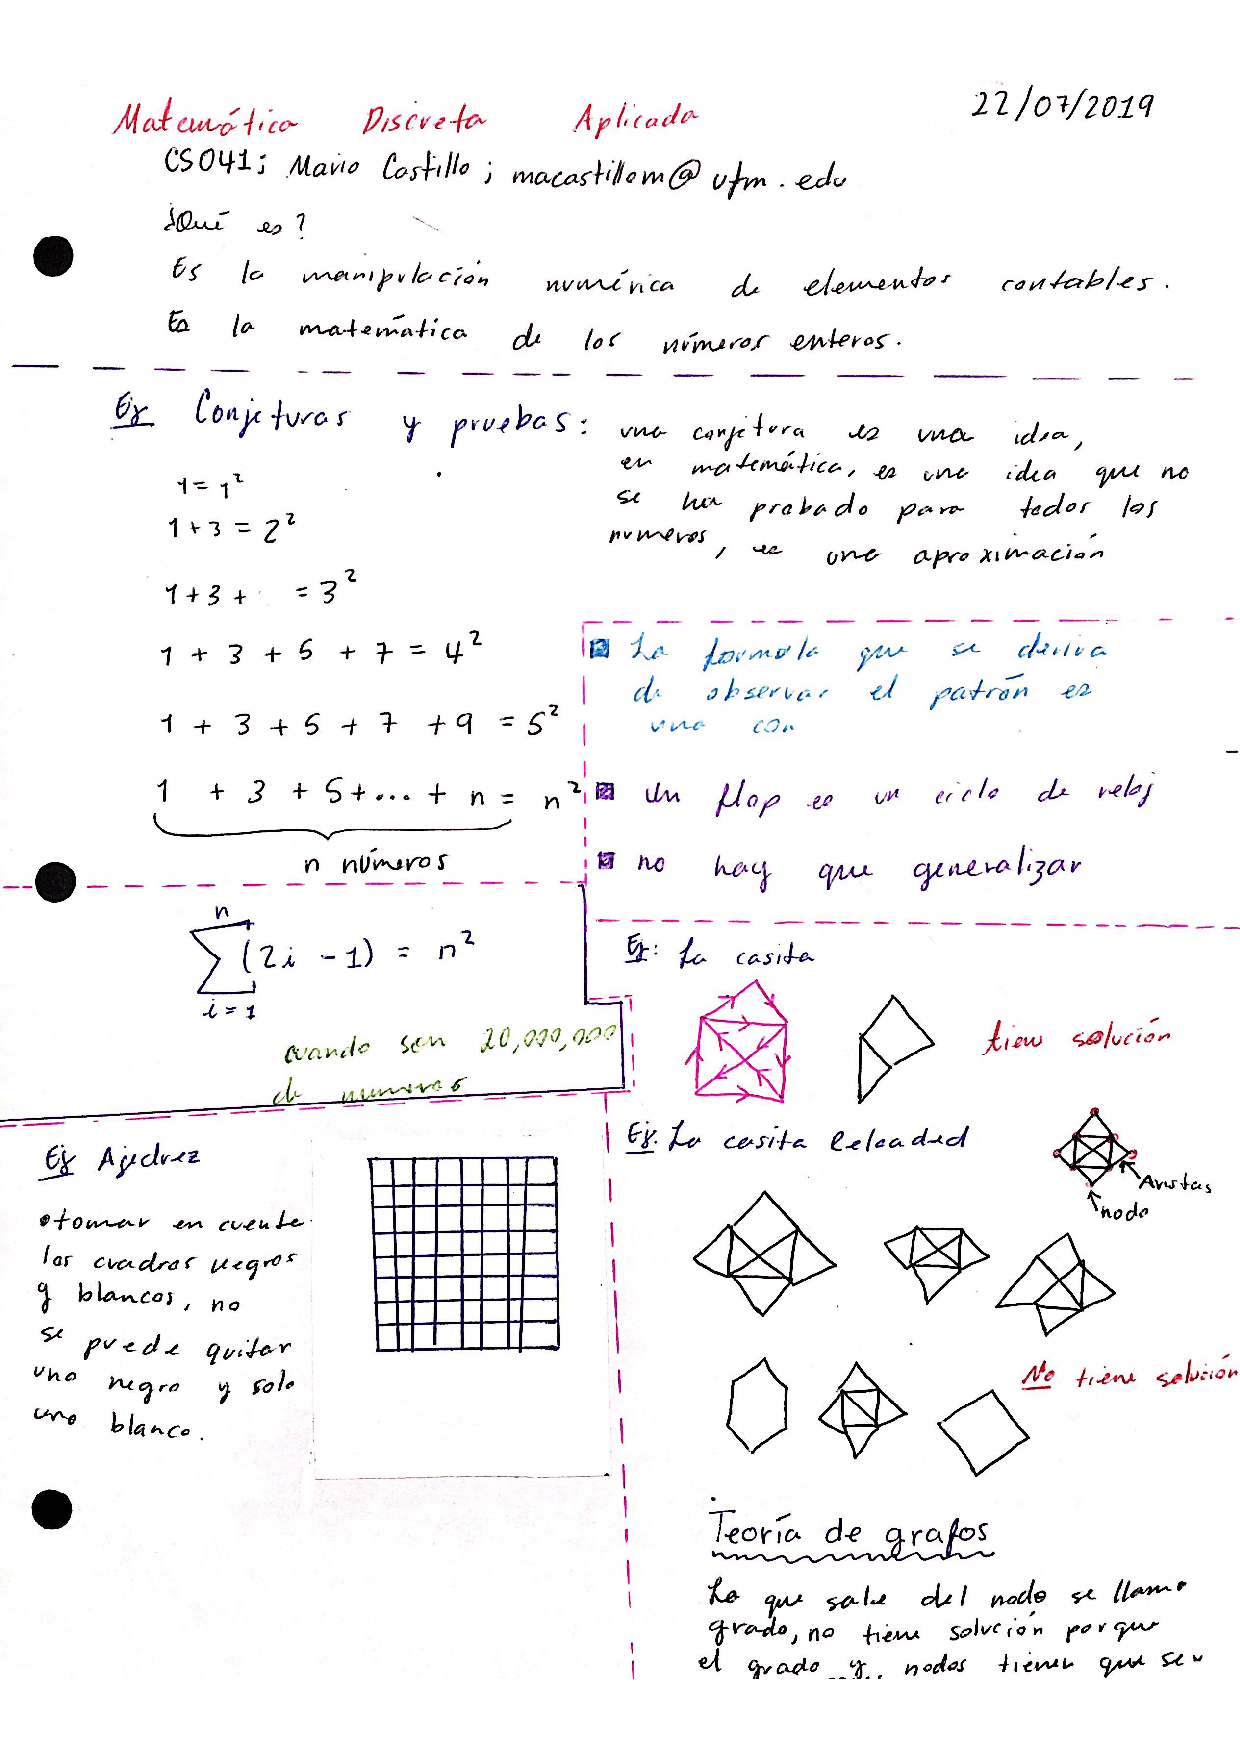
\includepdf[pages=-,pagecommand={\thispagestyle{plain}}]{Clases/2019-07-22.pdf}

\chapter{Clase del Día: 2019-07-24; Lógica proposicional, juegos de lógica más complejos, ejemplos de juegos de lógica}
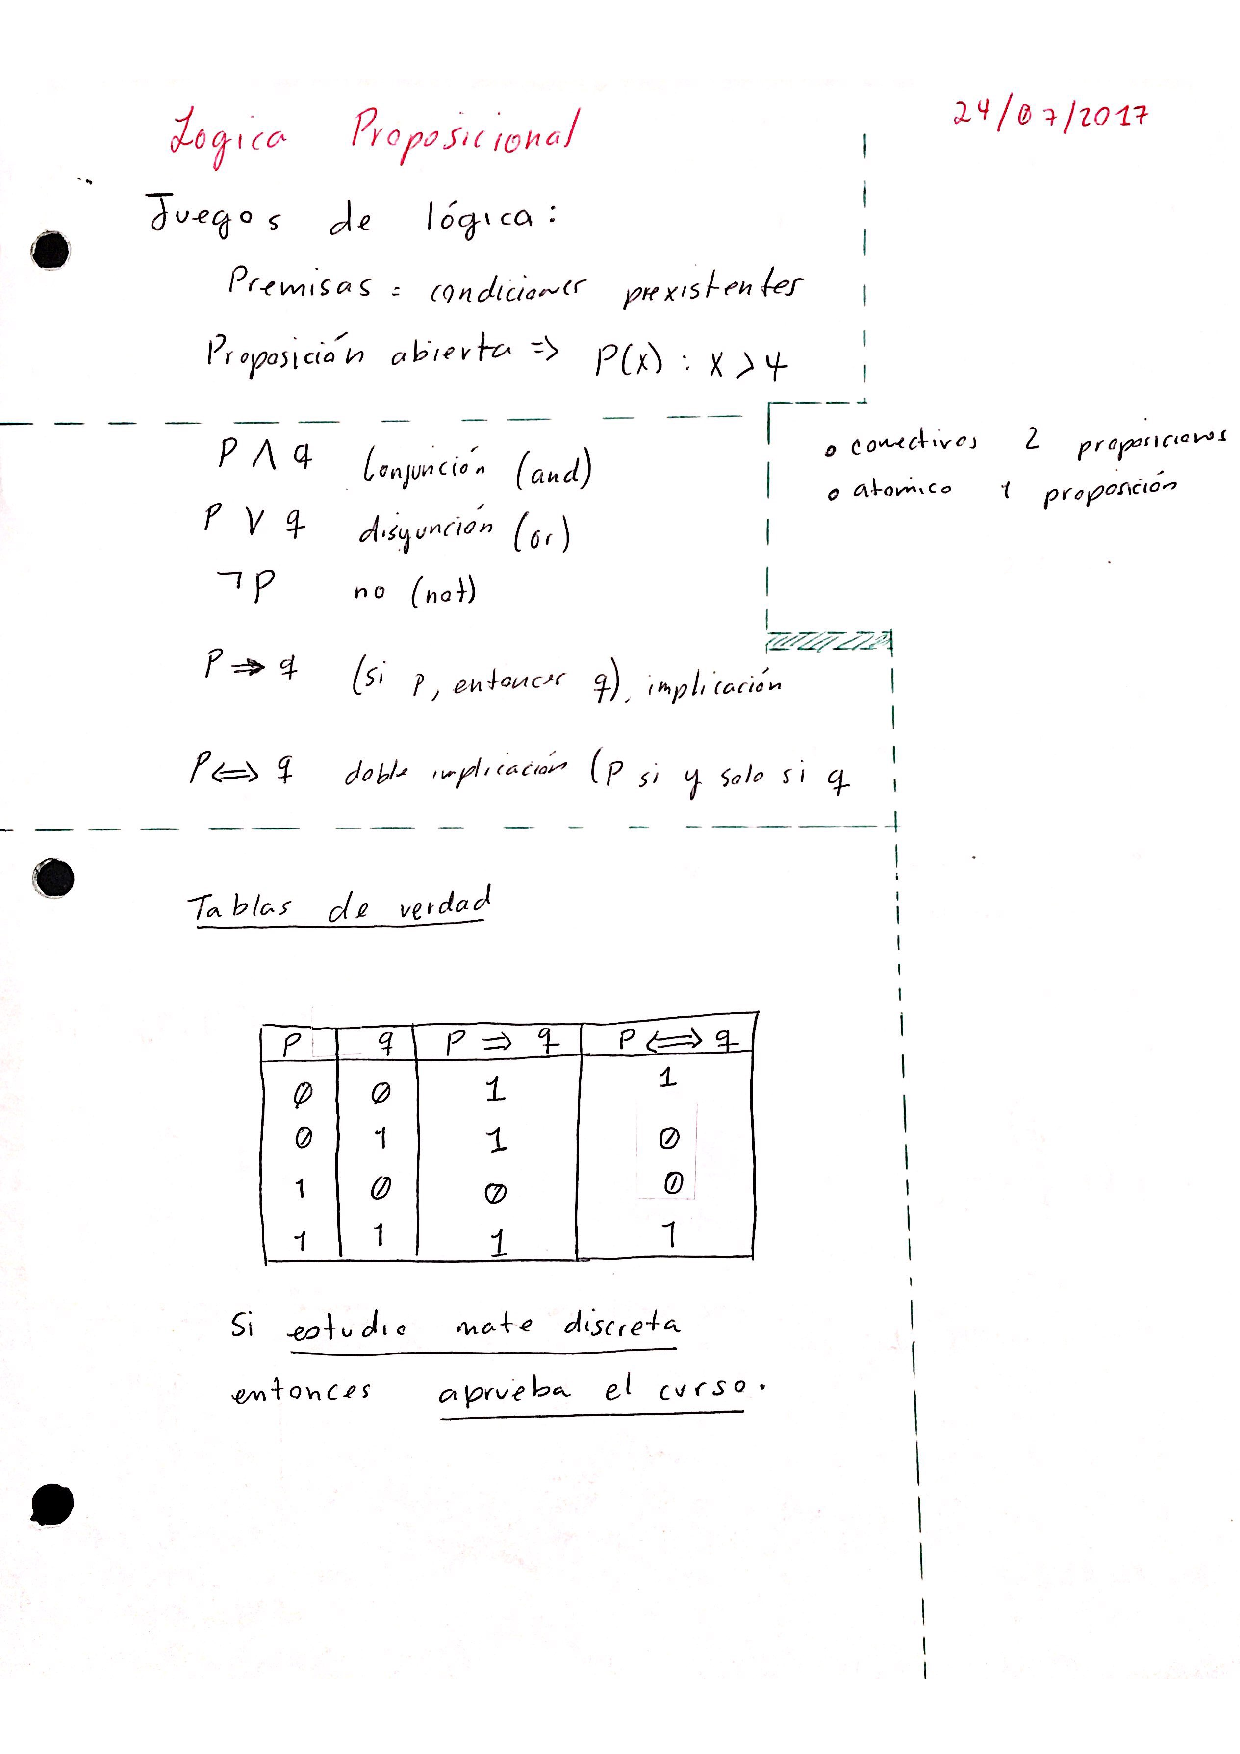
\includepdf[pages=-,pagecommand={\thispagestyle{plain}}]{Clases/2019-07-24.pdf}


\chapter{Clase del Día: 2019-07-29; Equivalencias lógicas, tautología, contradicción, contingencia, jerarquías operacionales lógicas}
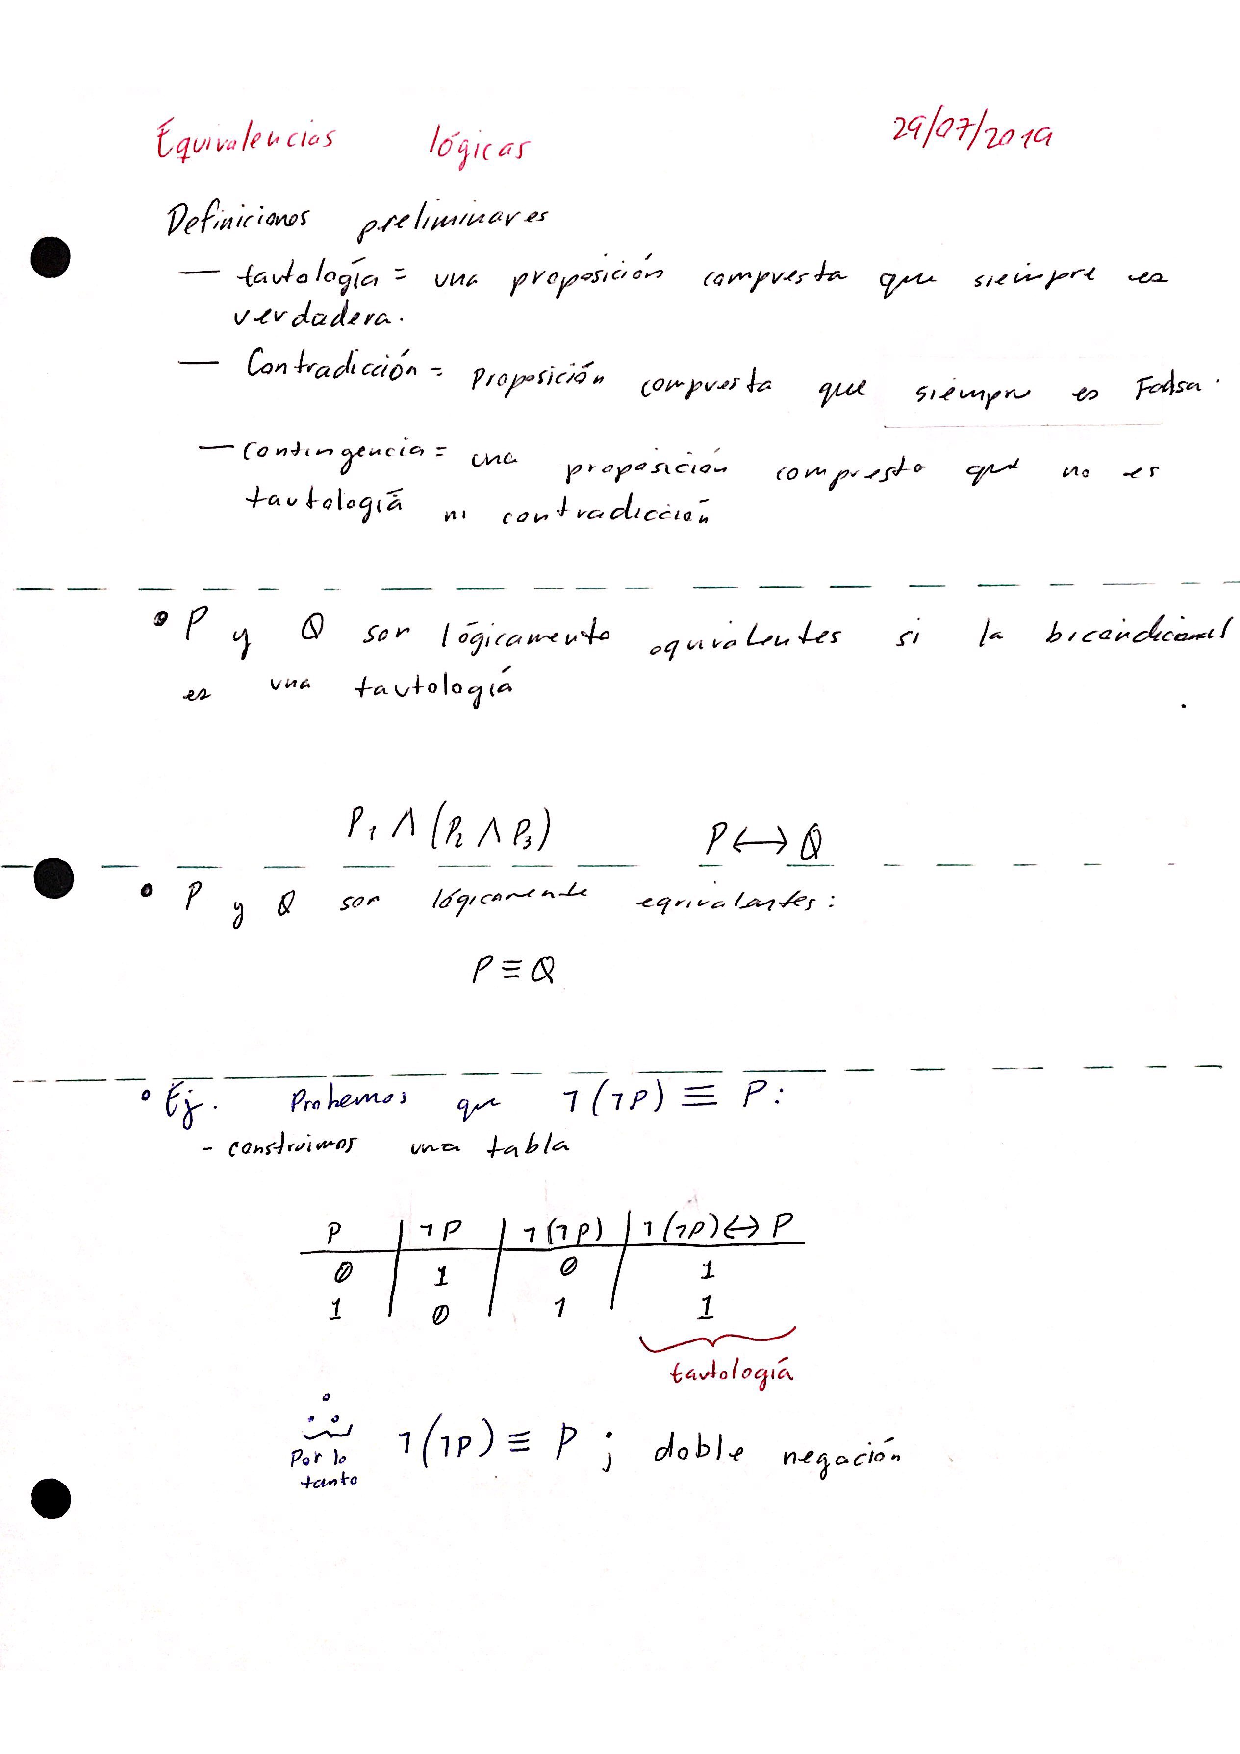
\includepdf[pages=-,pagecommand={\thispagestyle{plain}}]{Clases/2019-07-29.pdf}


\chapter{Clase del Día: 2019-07-31; Inferencia, reglas de inferencia, }
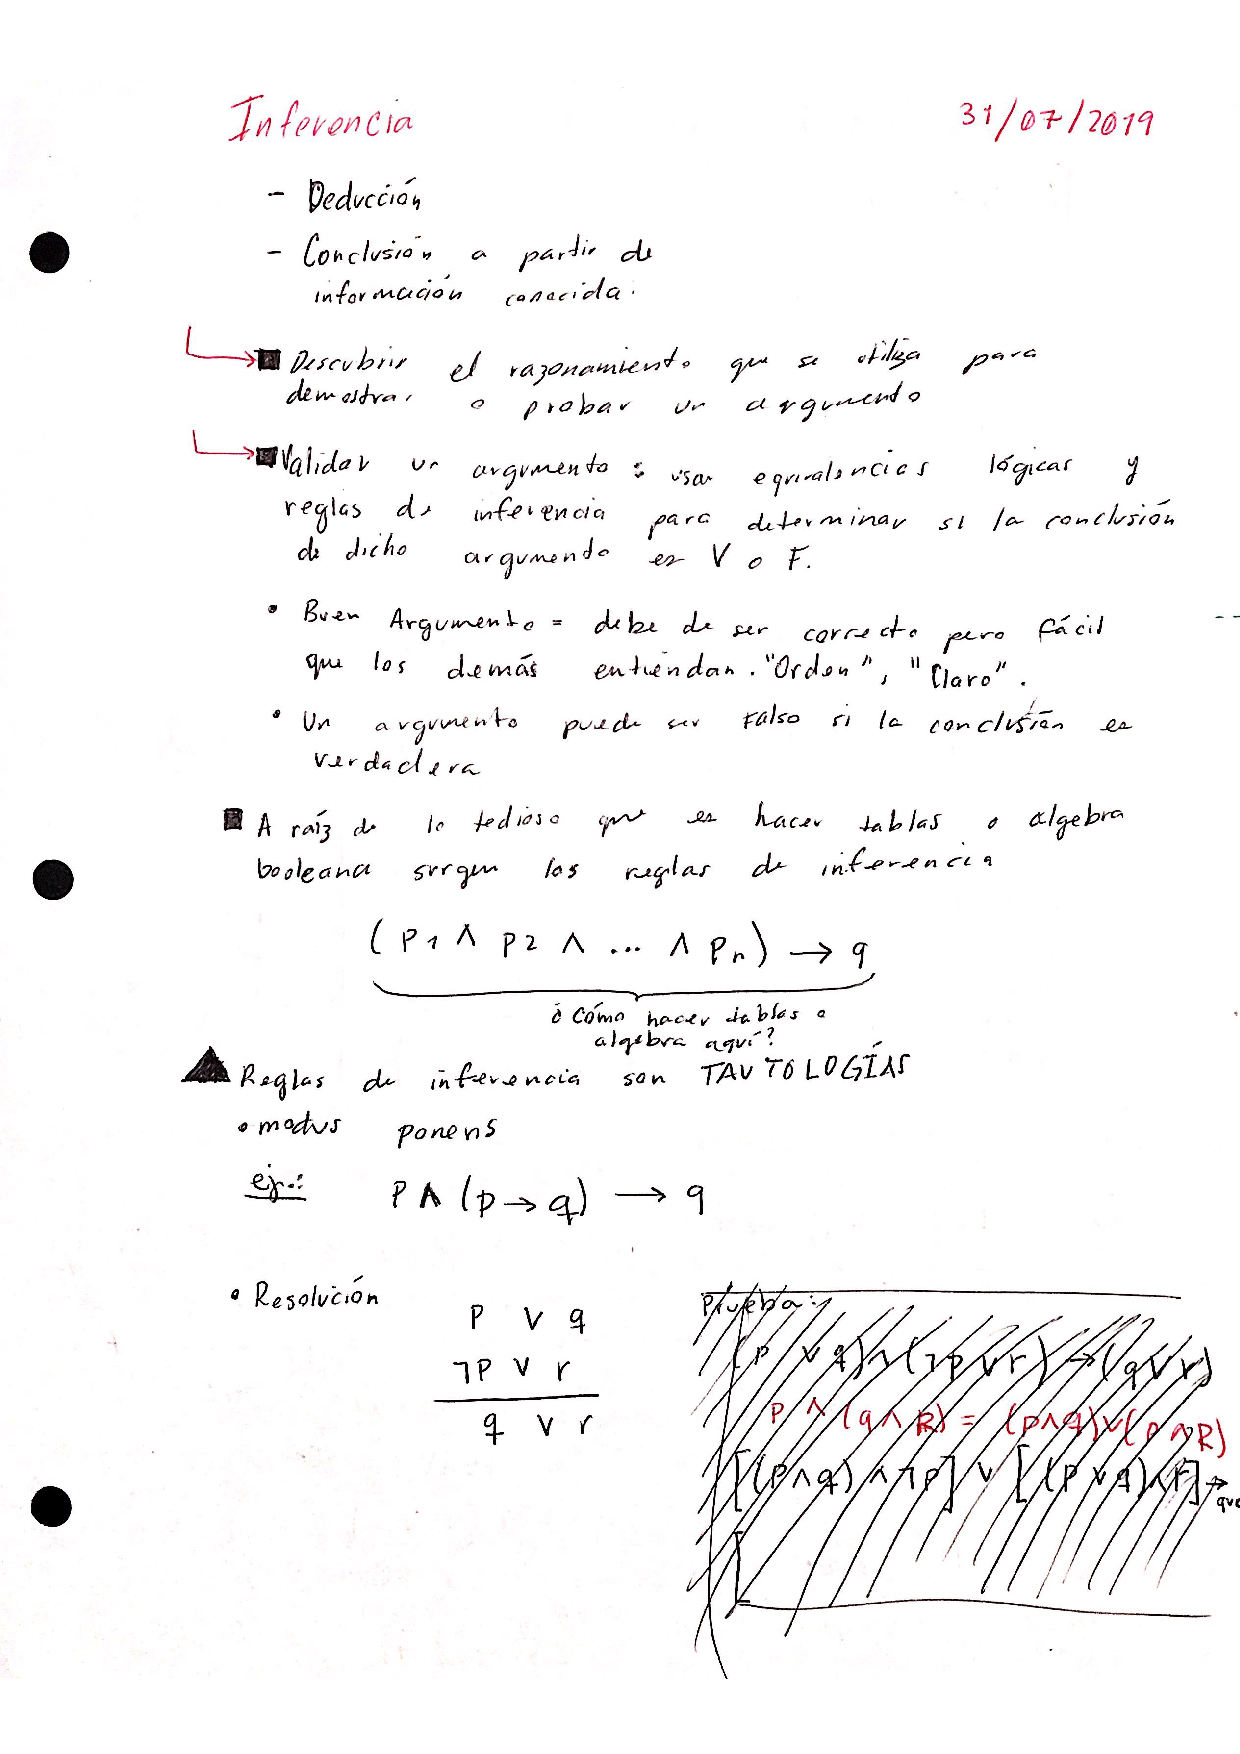
\includepdf[pages=-,pagecommand={\thispagestyle{plain}}]{Clases/2019-07-31.pdf}
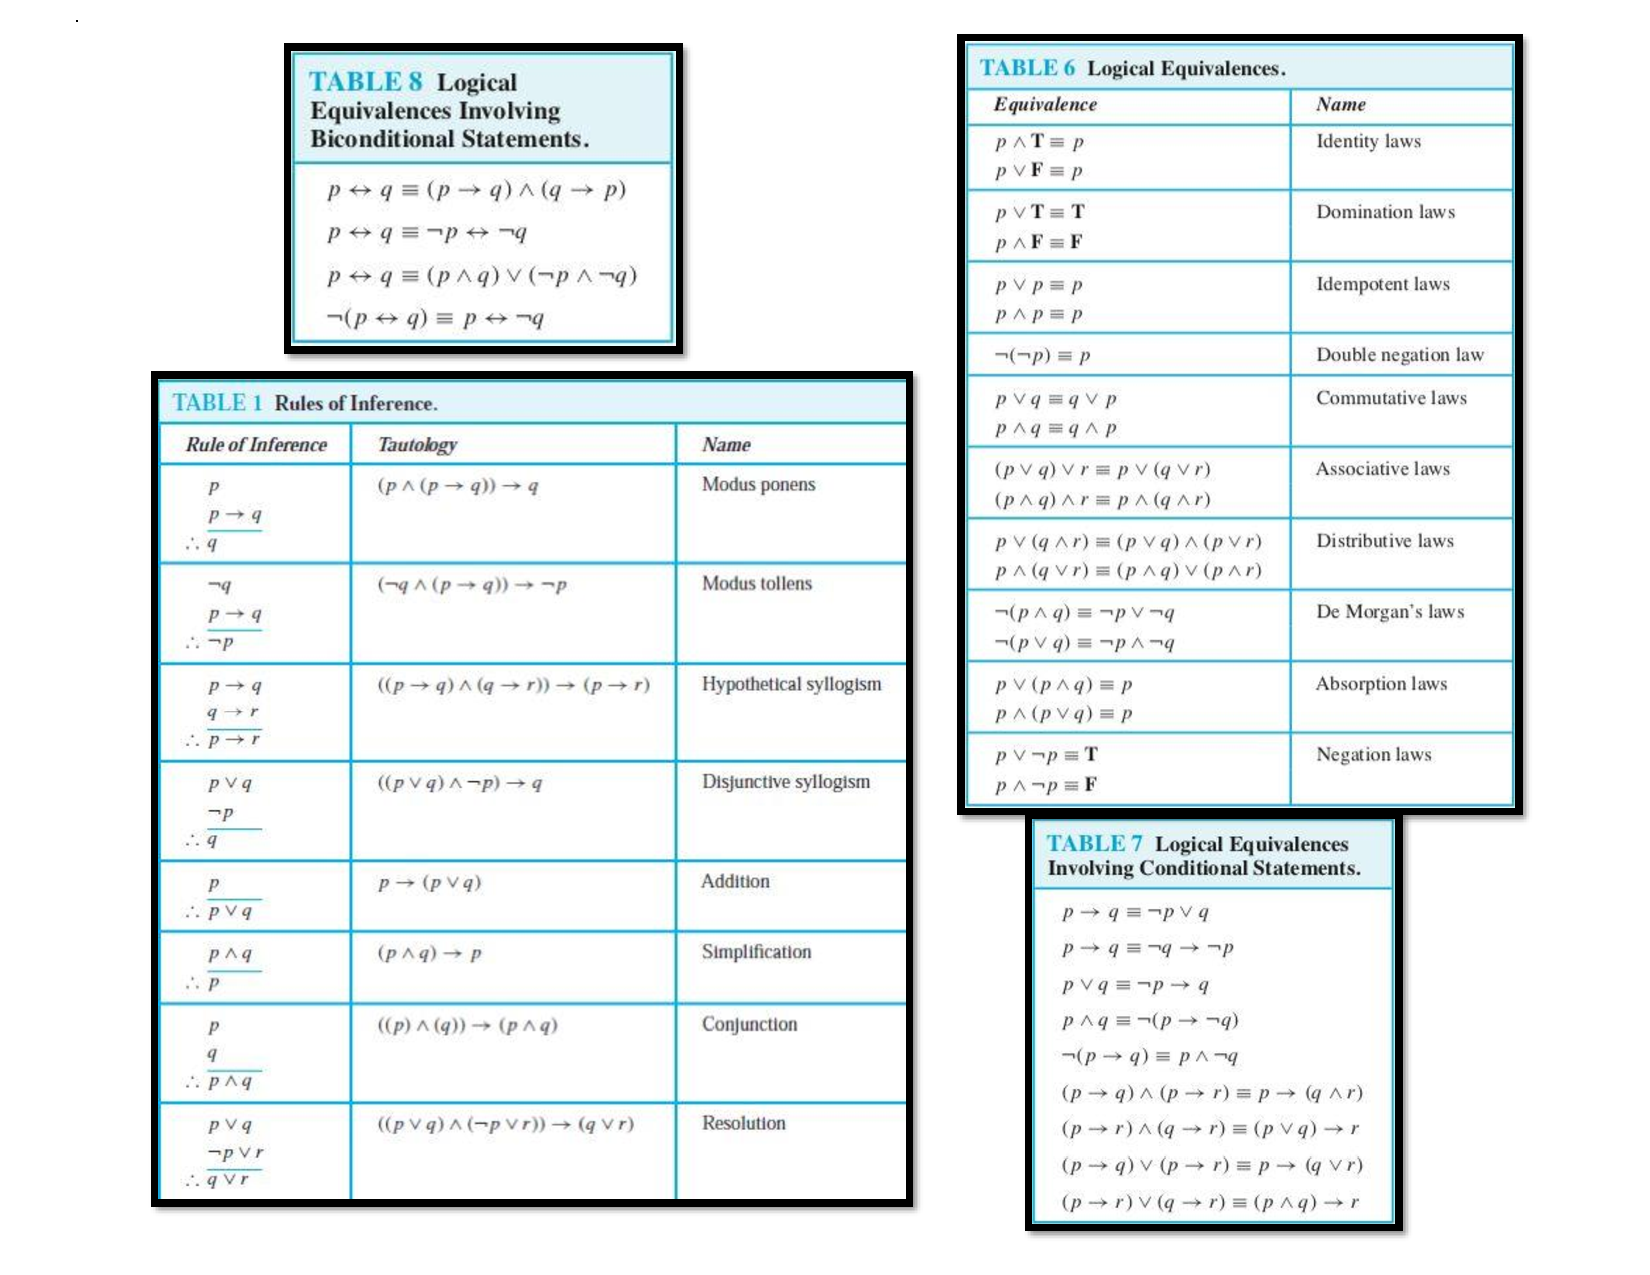
\includepdf[pages=-,pagecommand={\thispagestyle{plain}}]{pdf/F.pdf}


\chapter{Clase del Día: 2019-08-05; Primer laboratorio de lógica proposicional, equivalencias lógicas, reglas de inferencia}
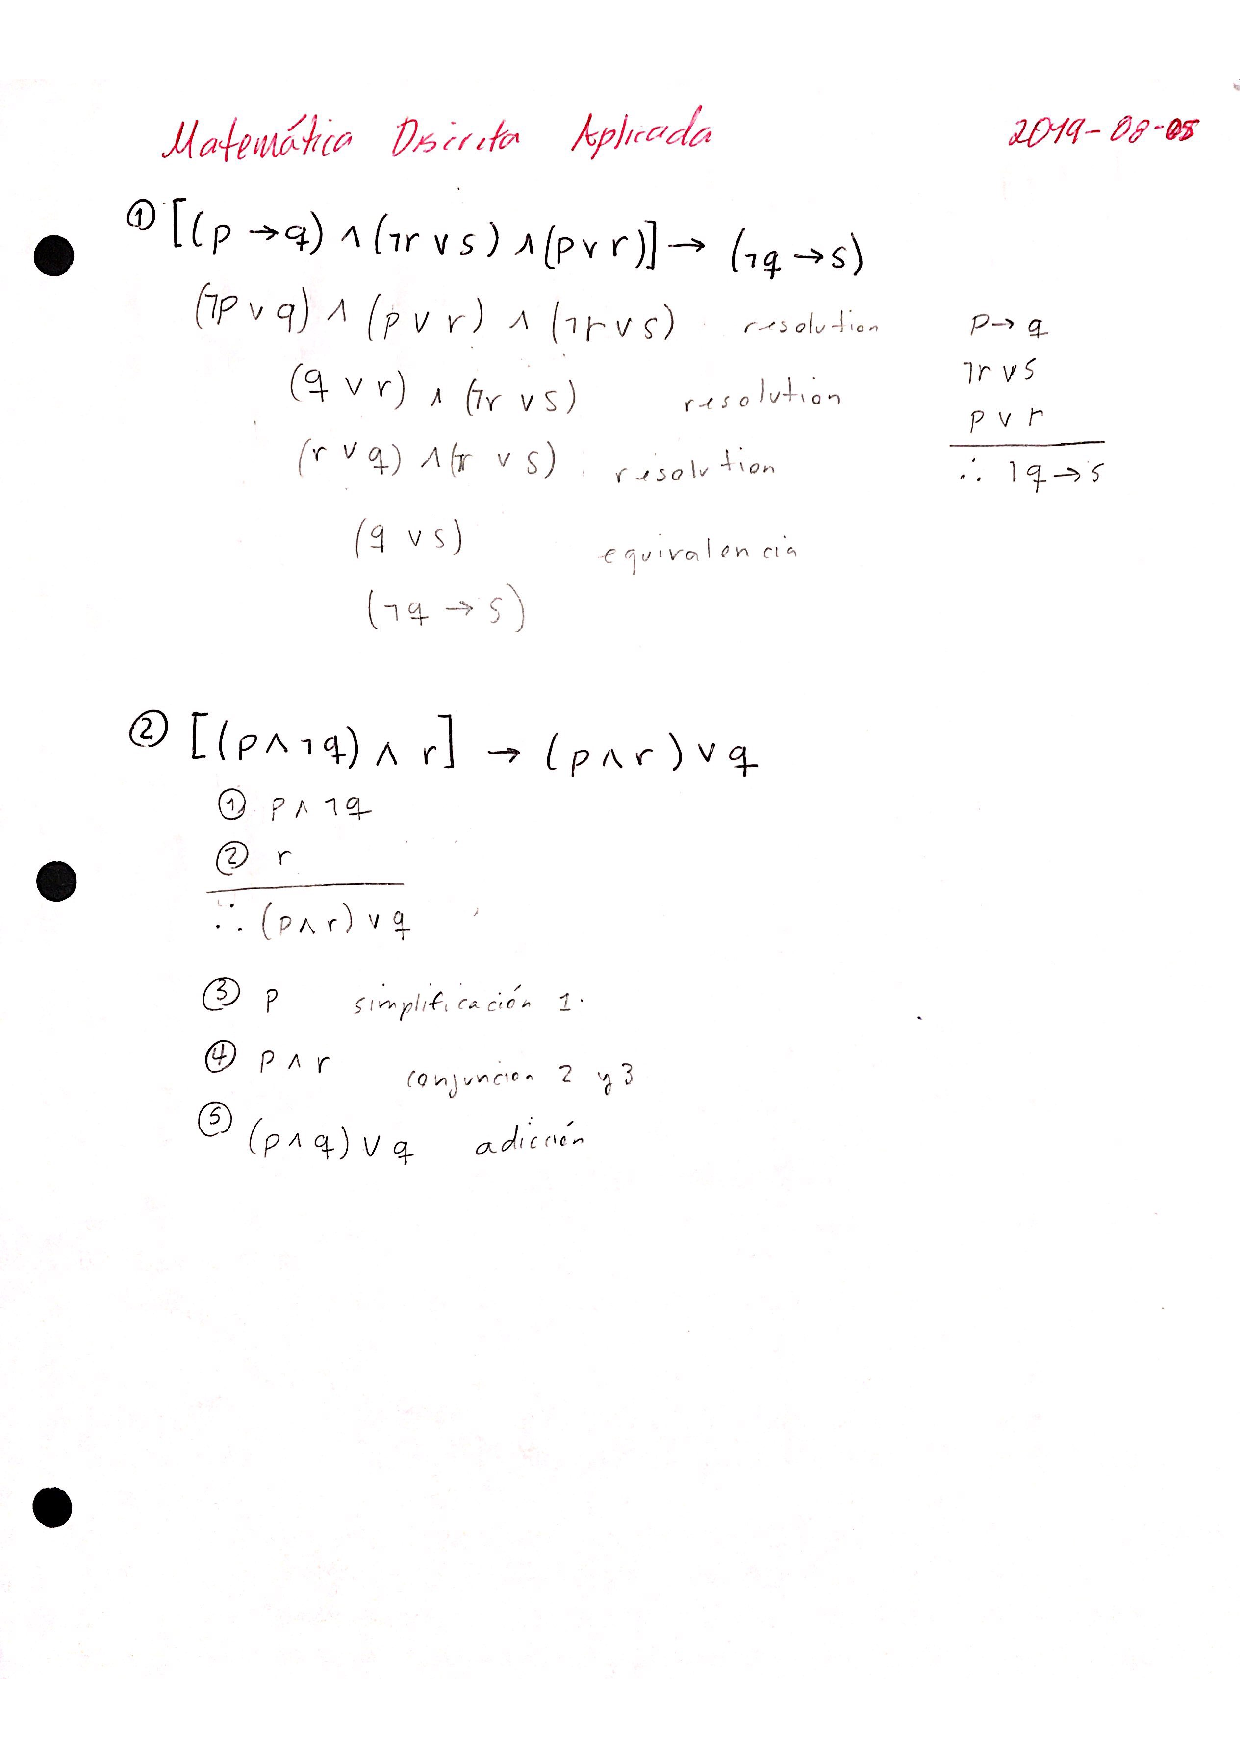
\includepdf[pages=-,pagecommand={\thispagestyle{plain}}]{Clases/2019-08-05.pdf}


\chapter{Clase del Día: 2019-08-07; Técnicas de demostración, prueba directa, sets de números}
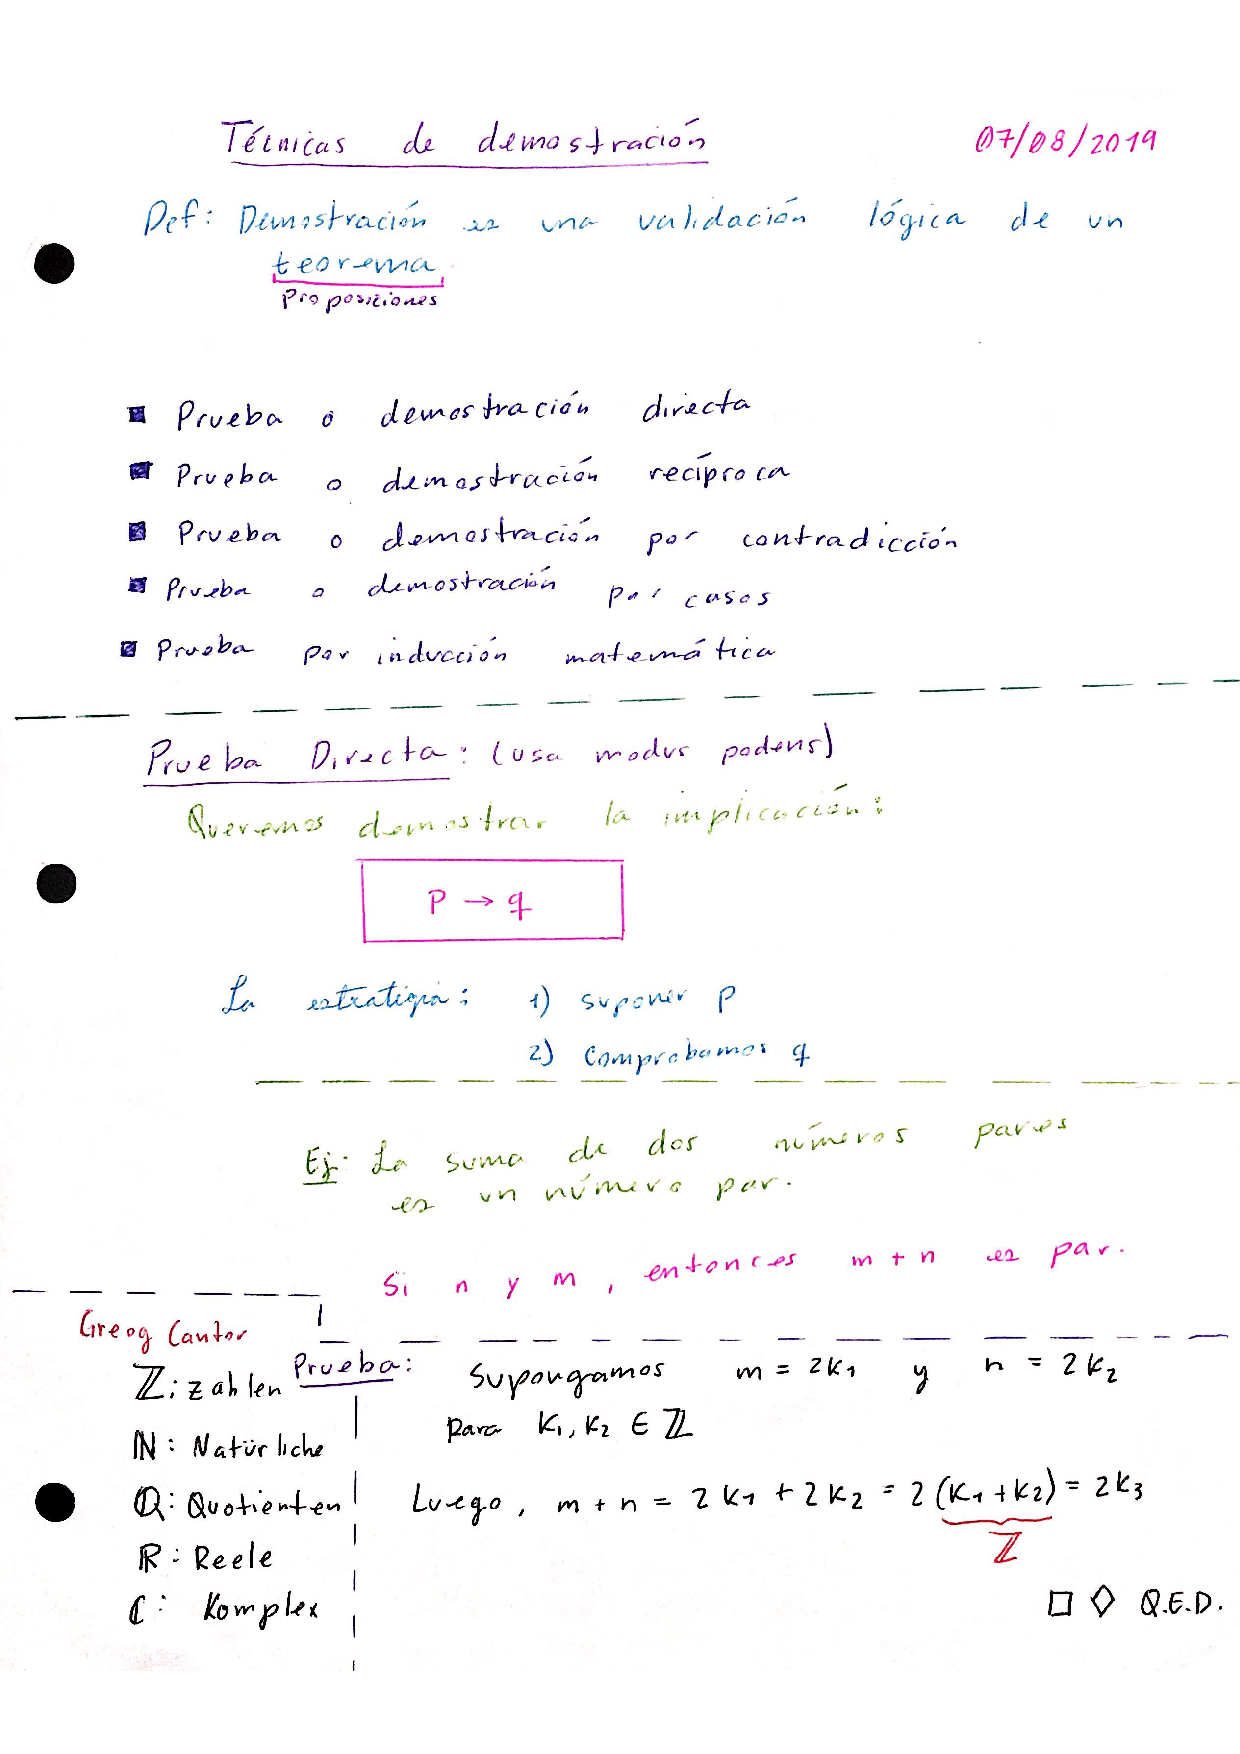
\includepdf[pages=-,pagecommand={\thispagestyle{plain}}]{Clases/2019-08-07.pdf}


\chapter{Clase del Día: 2019-08-12; Continuación de técnicas de demostración, prueba directa, prueba por contra-recíproca, prueba por casos(exhausión), prueba por contradicción}
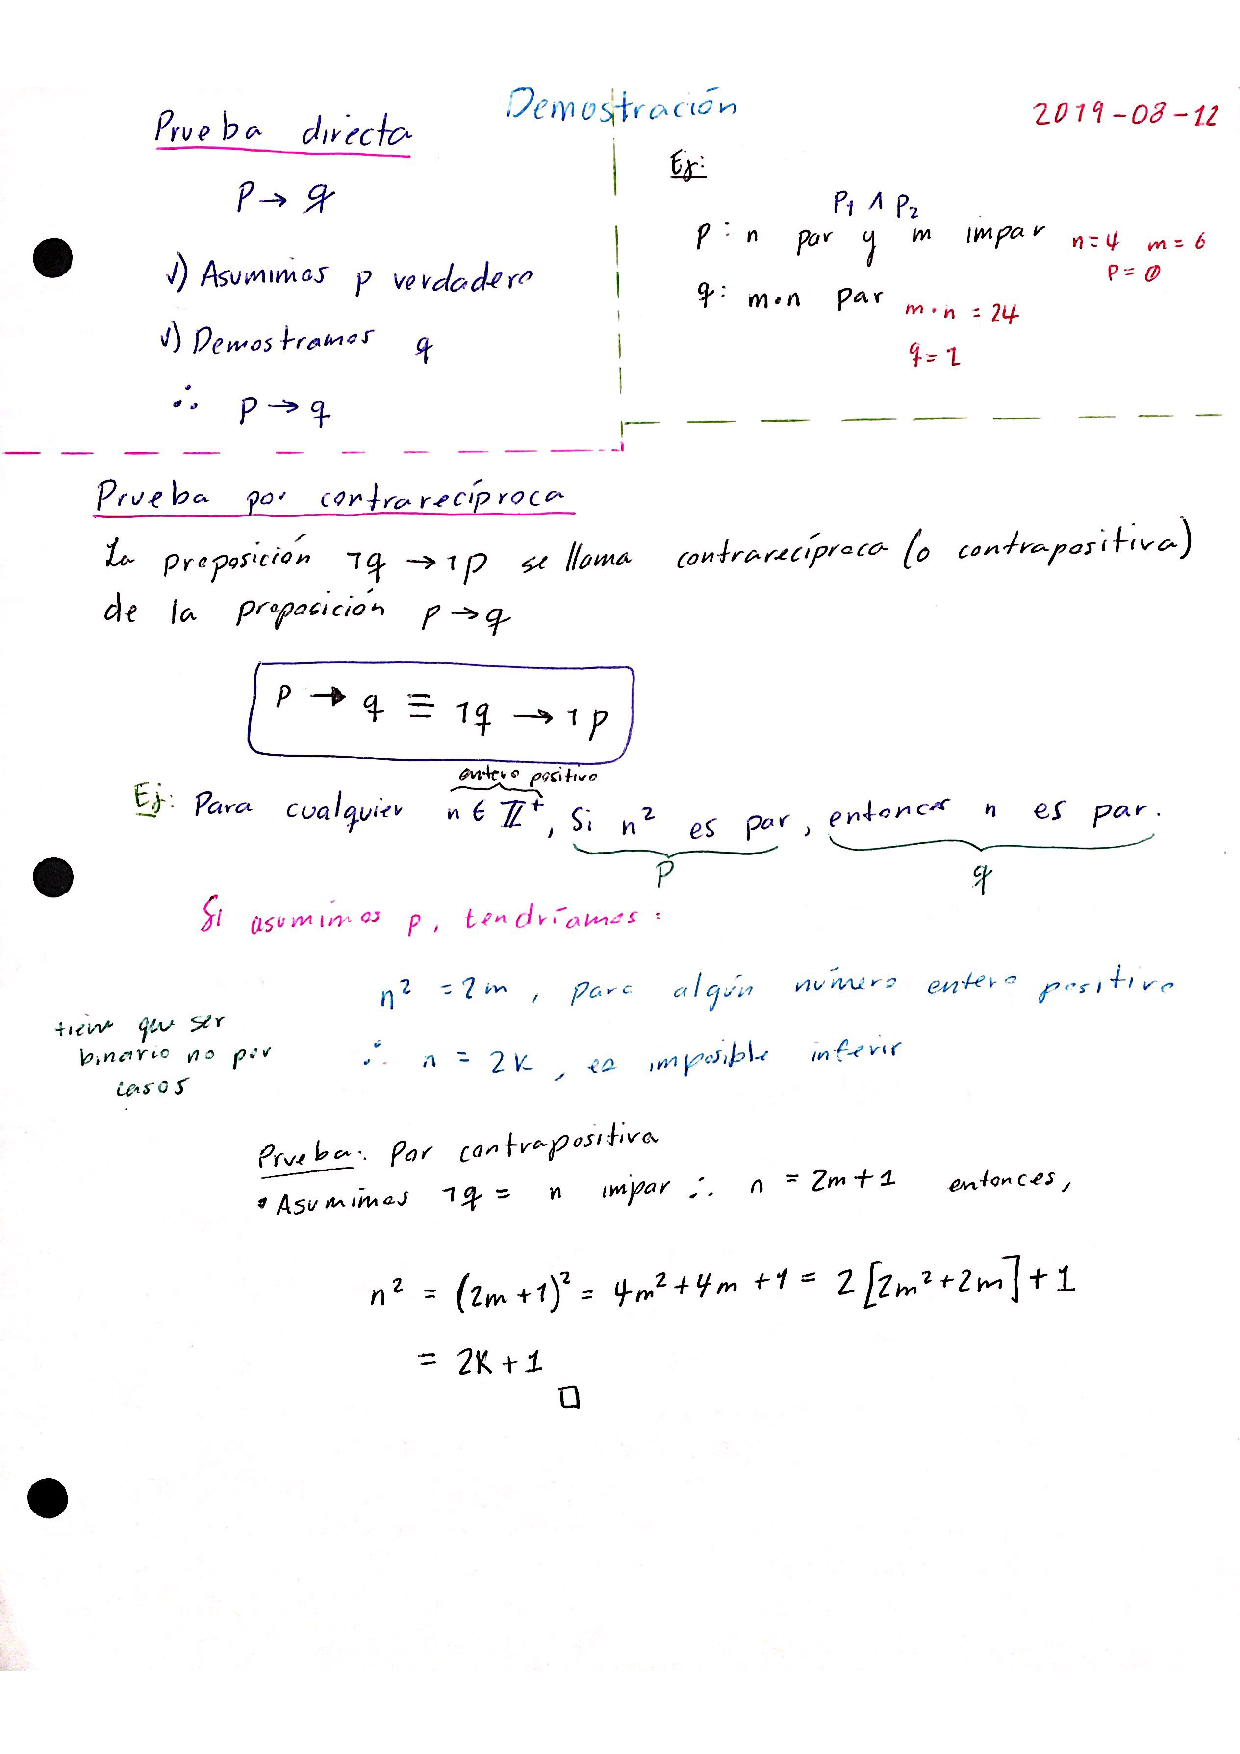
\includepdf[pages=-,pagecommand={\thispagestyle{plain}}]{Clases/2019-08-12.pdf}


\chapter{Clase del Día: 2019-08-14; Más ejemplos de técnicas de demostración, introducción a la \textbf{inducción matemática}}
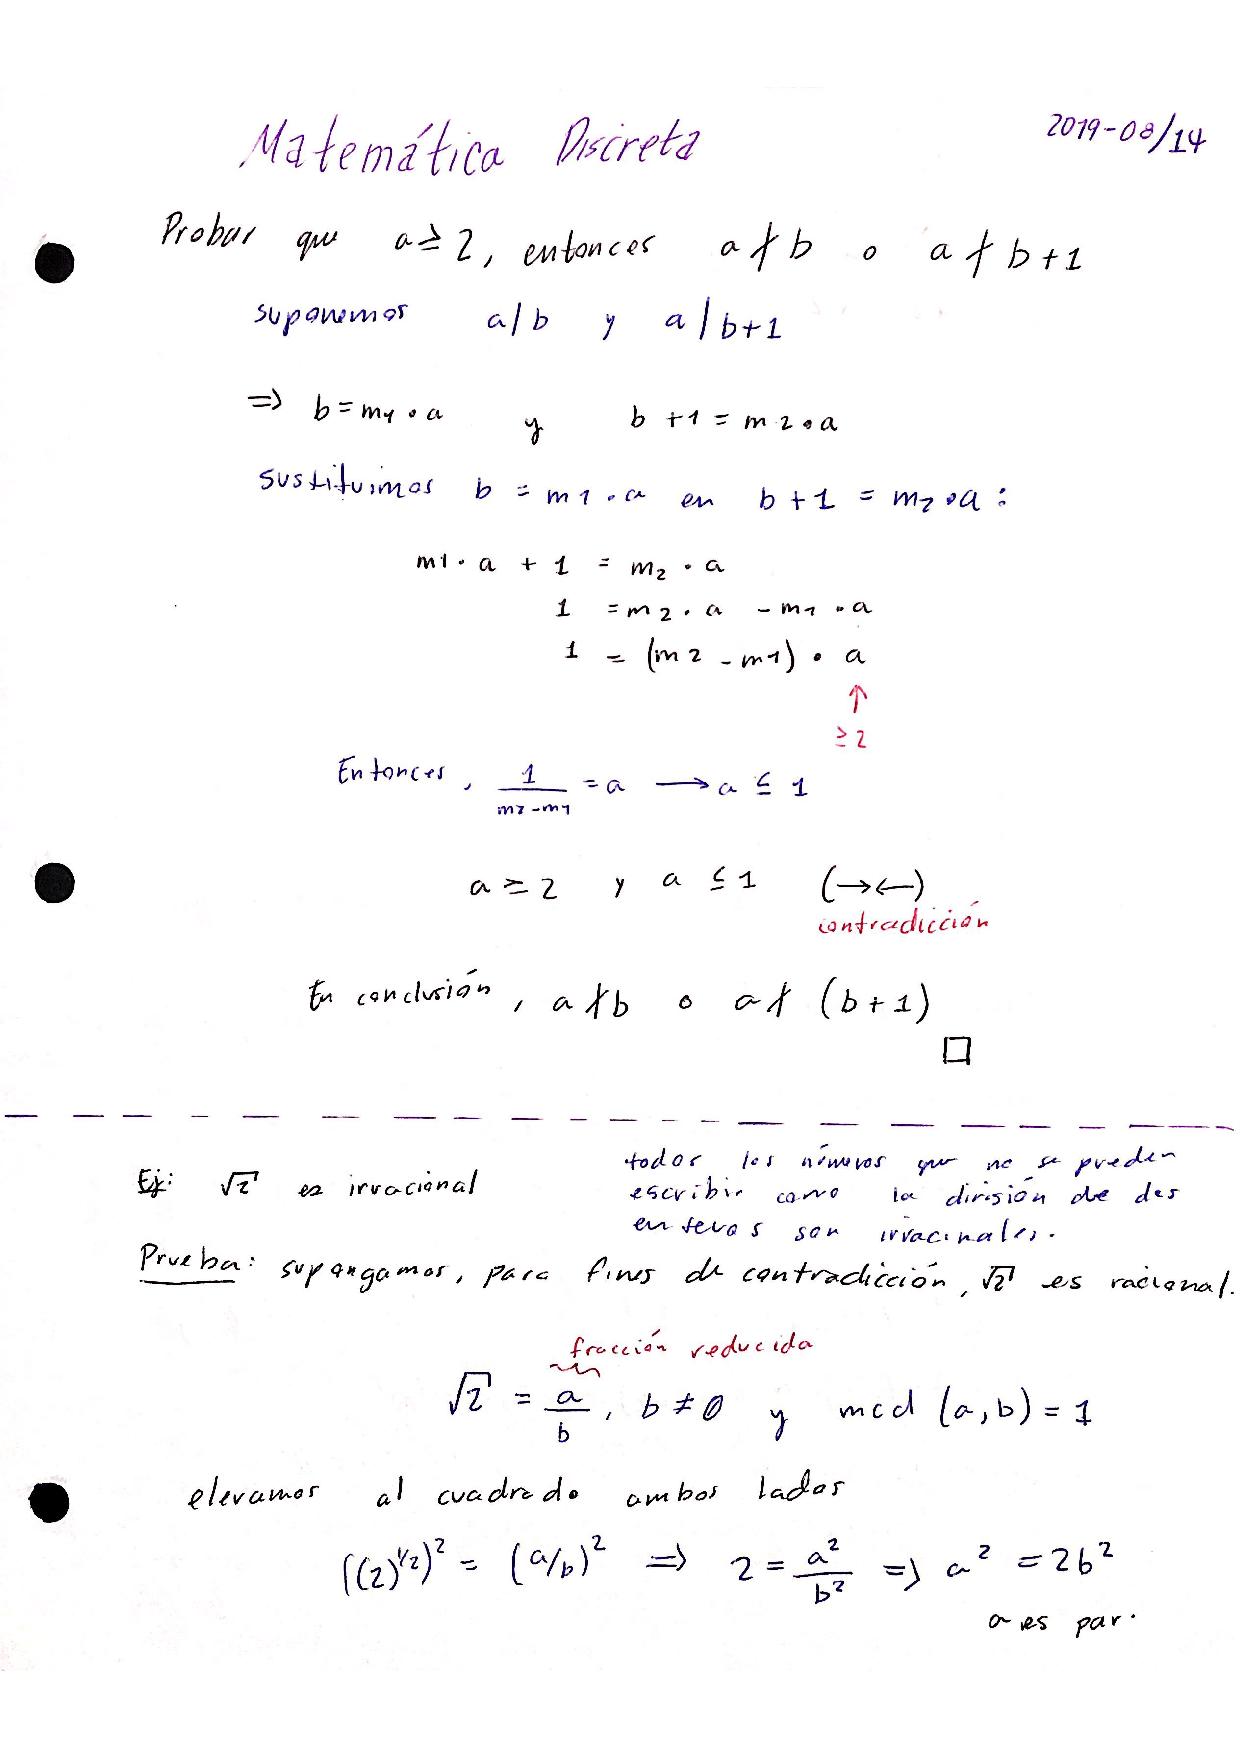
\includepdf[pages=-,pagecommand={\thispagestyle{plain}}]{Clases/2019-08-14.pdf}


\chapter{Clase del Día: 2019-08-19; Continuación inducción
matemática, más ejemplos con las técnicas de demostración presentadas hasta el momento, \textbf{técnicas de conteo}, principio de la suma, principio del producto}
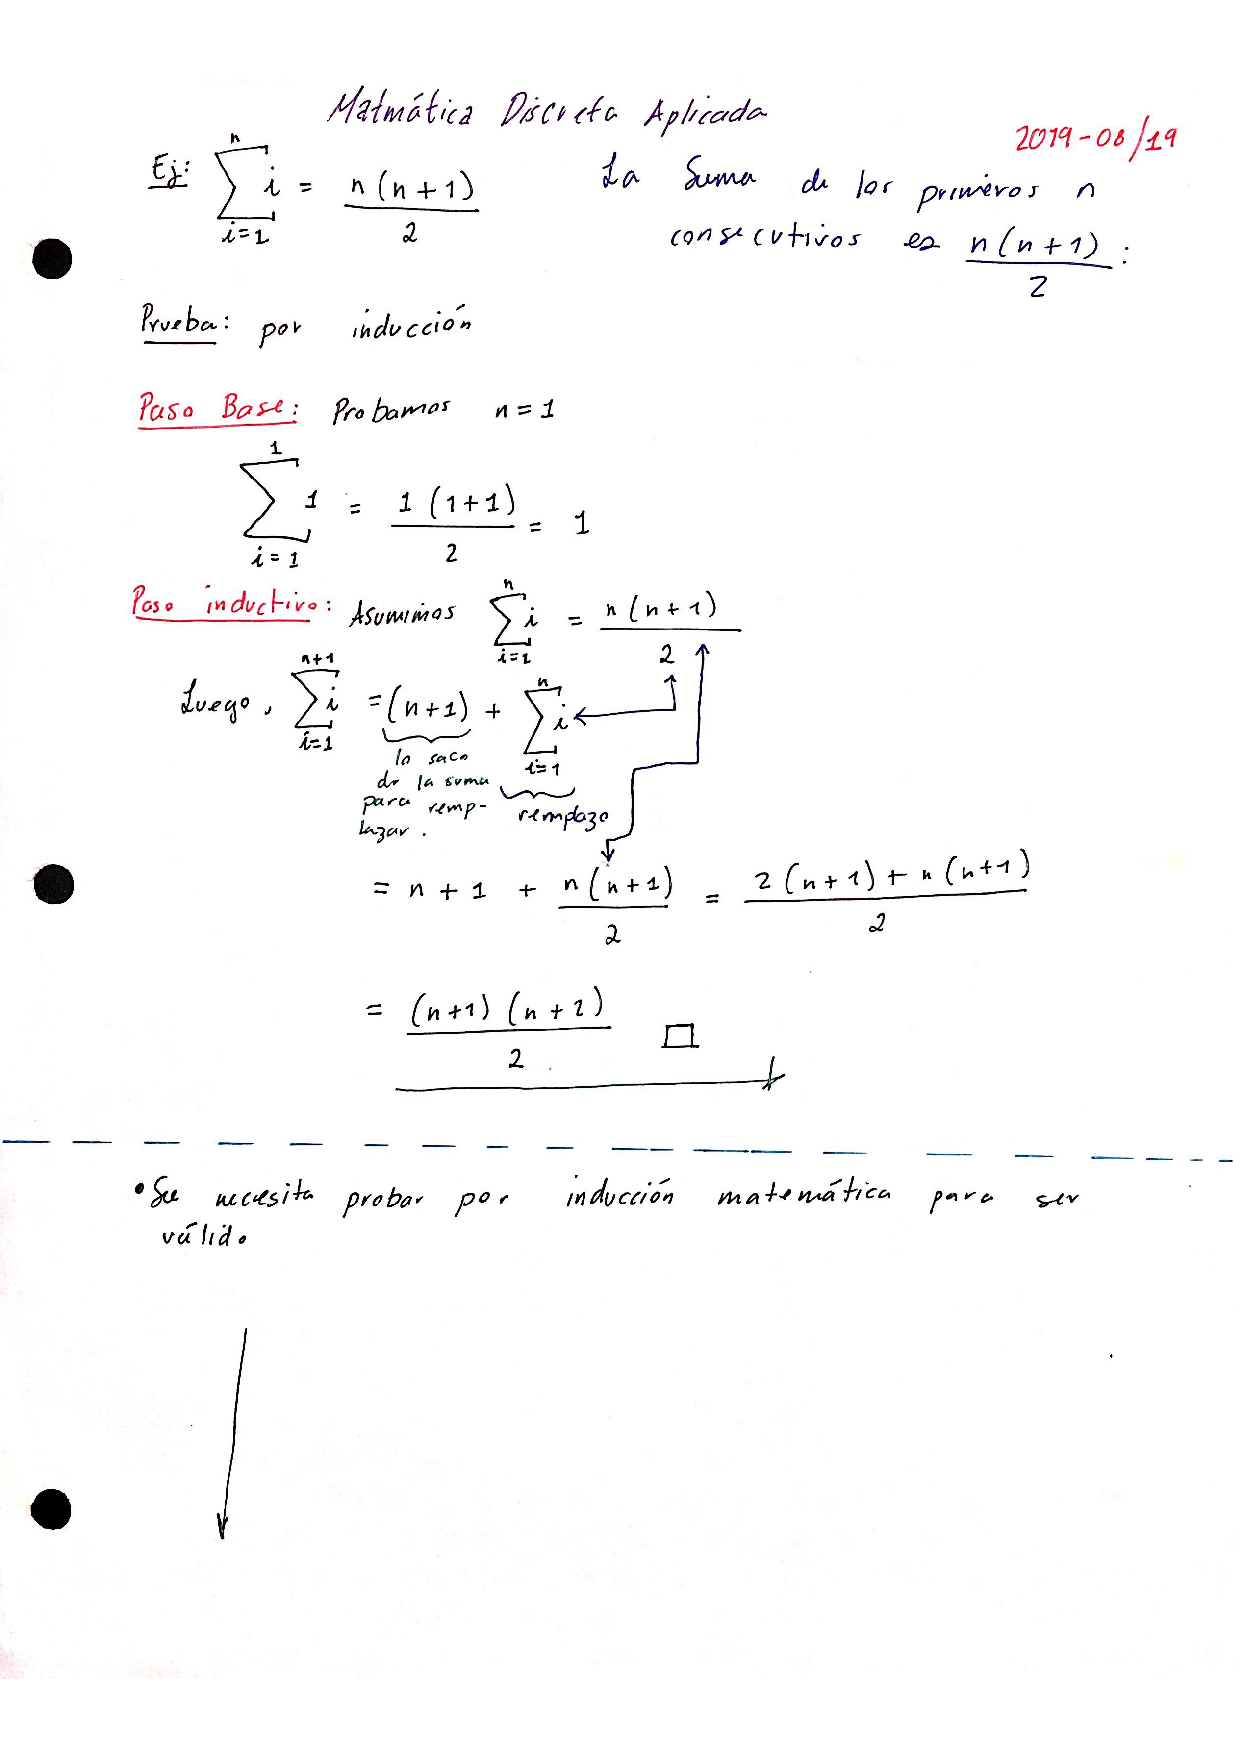
\includepdf[pages=-,pagecommand={\thispagestyle{plain}}]{Clases/2019-08-19.pdf}


\chapter{Clase del Día: 2019-08-21; definición de P.S. \$ P.P., ejemplos, ¿cómo complementan estos principios a las técnicas de demostración?, \textbf{Permutaciones}}
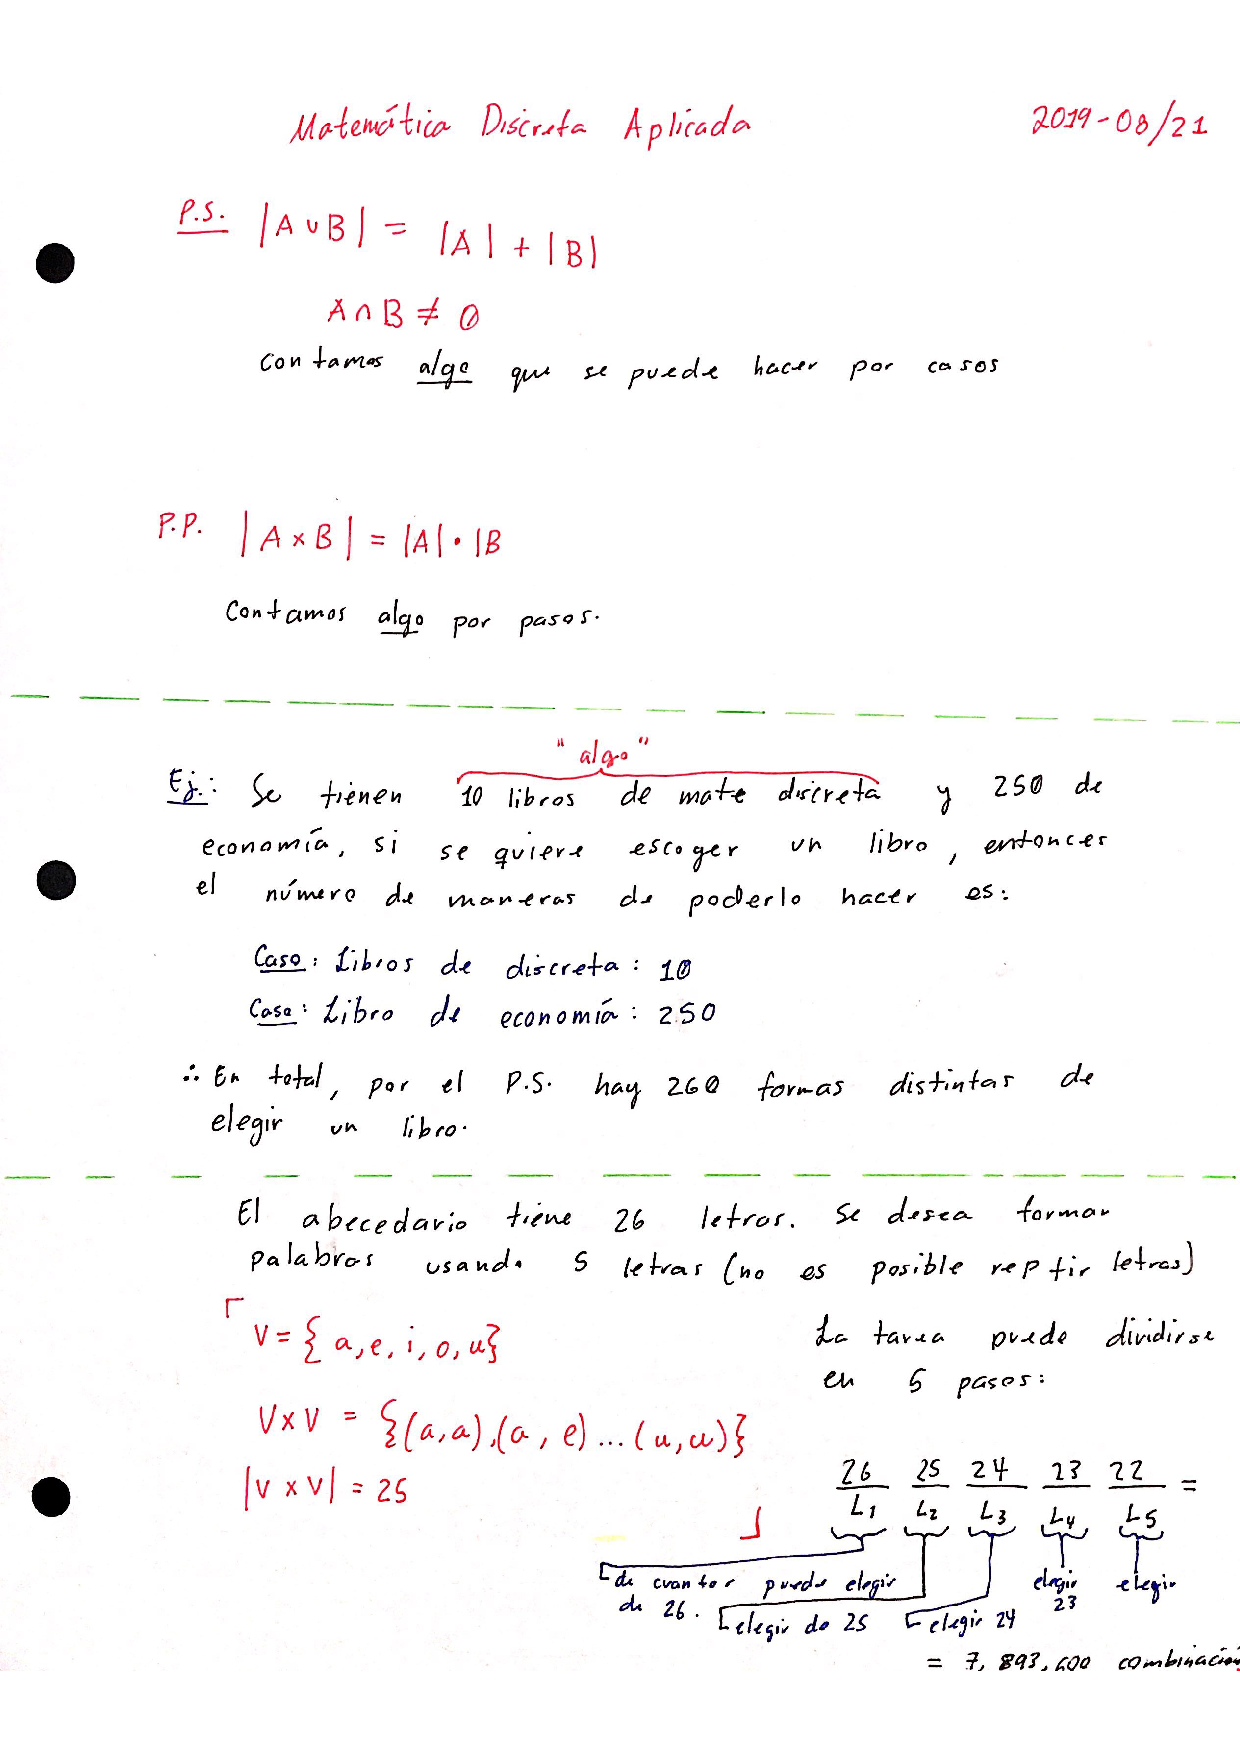
\includepdf[pages=-,pagecommand={\thispagestyle{plain}}]{Clases/2019-08-21.pdf}

\chapter{Clase del Día: 2019-08-26; Combinatoria, ejercicios con Álvaro}
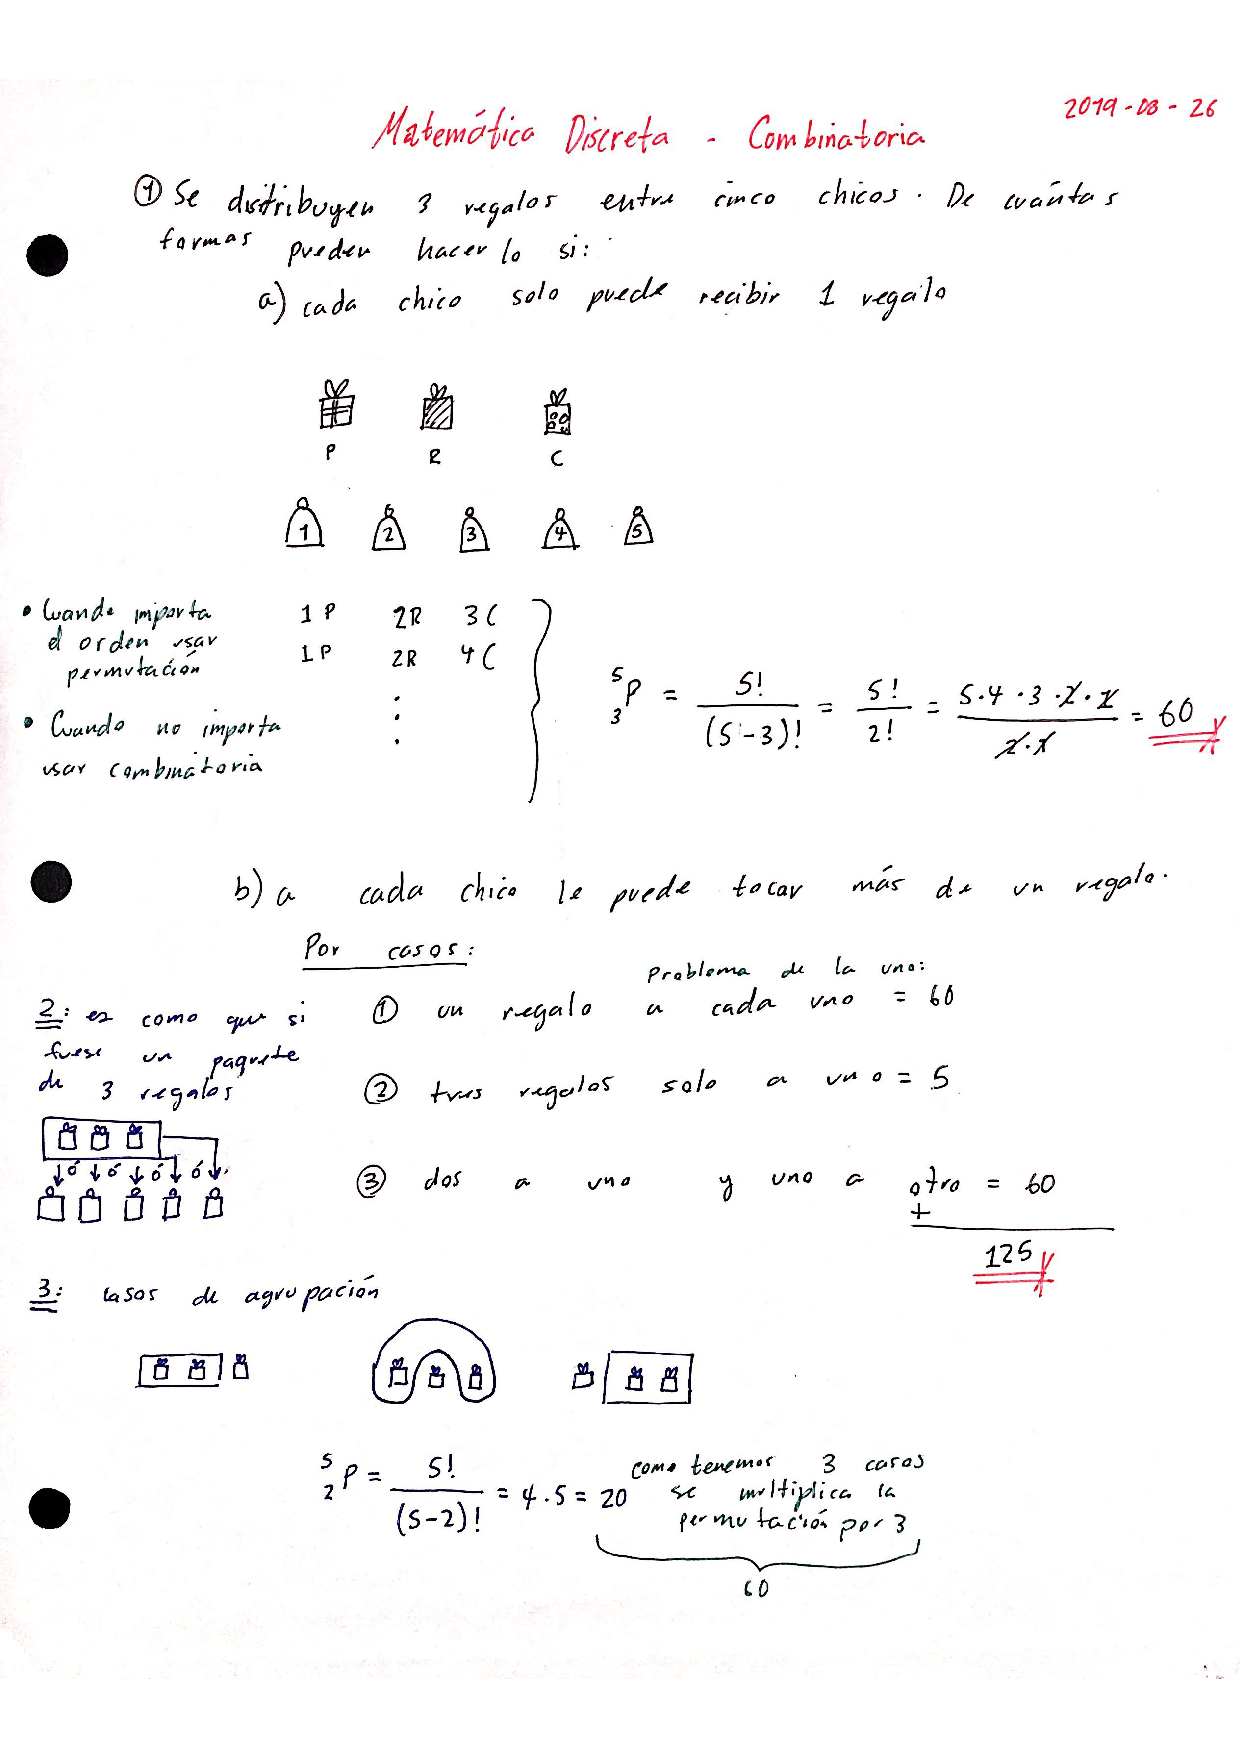
\includepdf[pages=-,pagecommand={\thispagestyle{plain}}]{Clases/2019-08-26.pdf}

\chapter{Clase del Día: 2019-08-28, Combinaciónes, ejemplos}
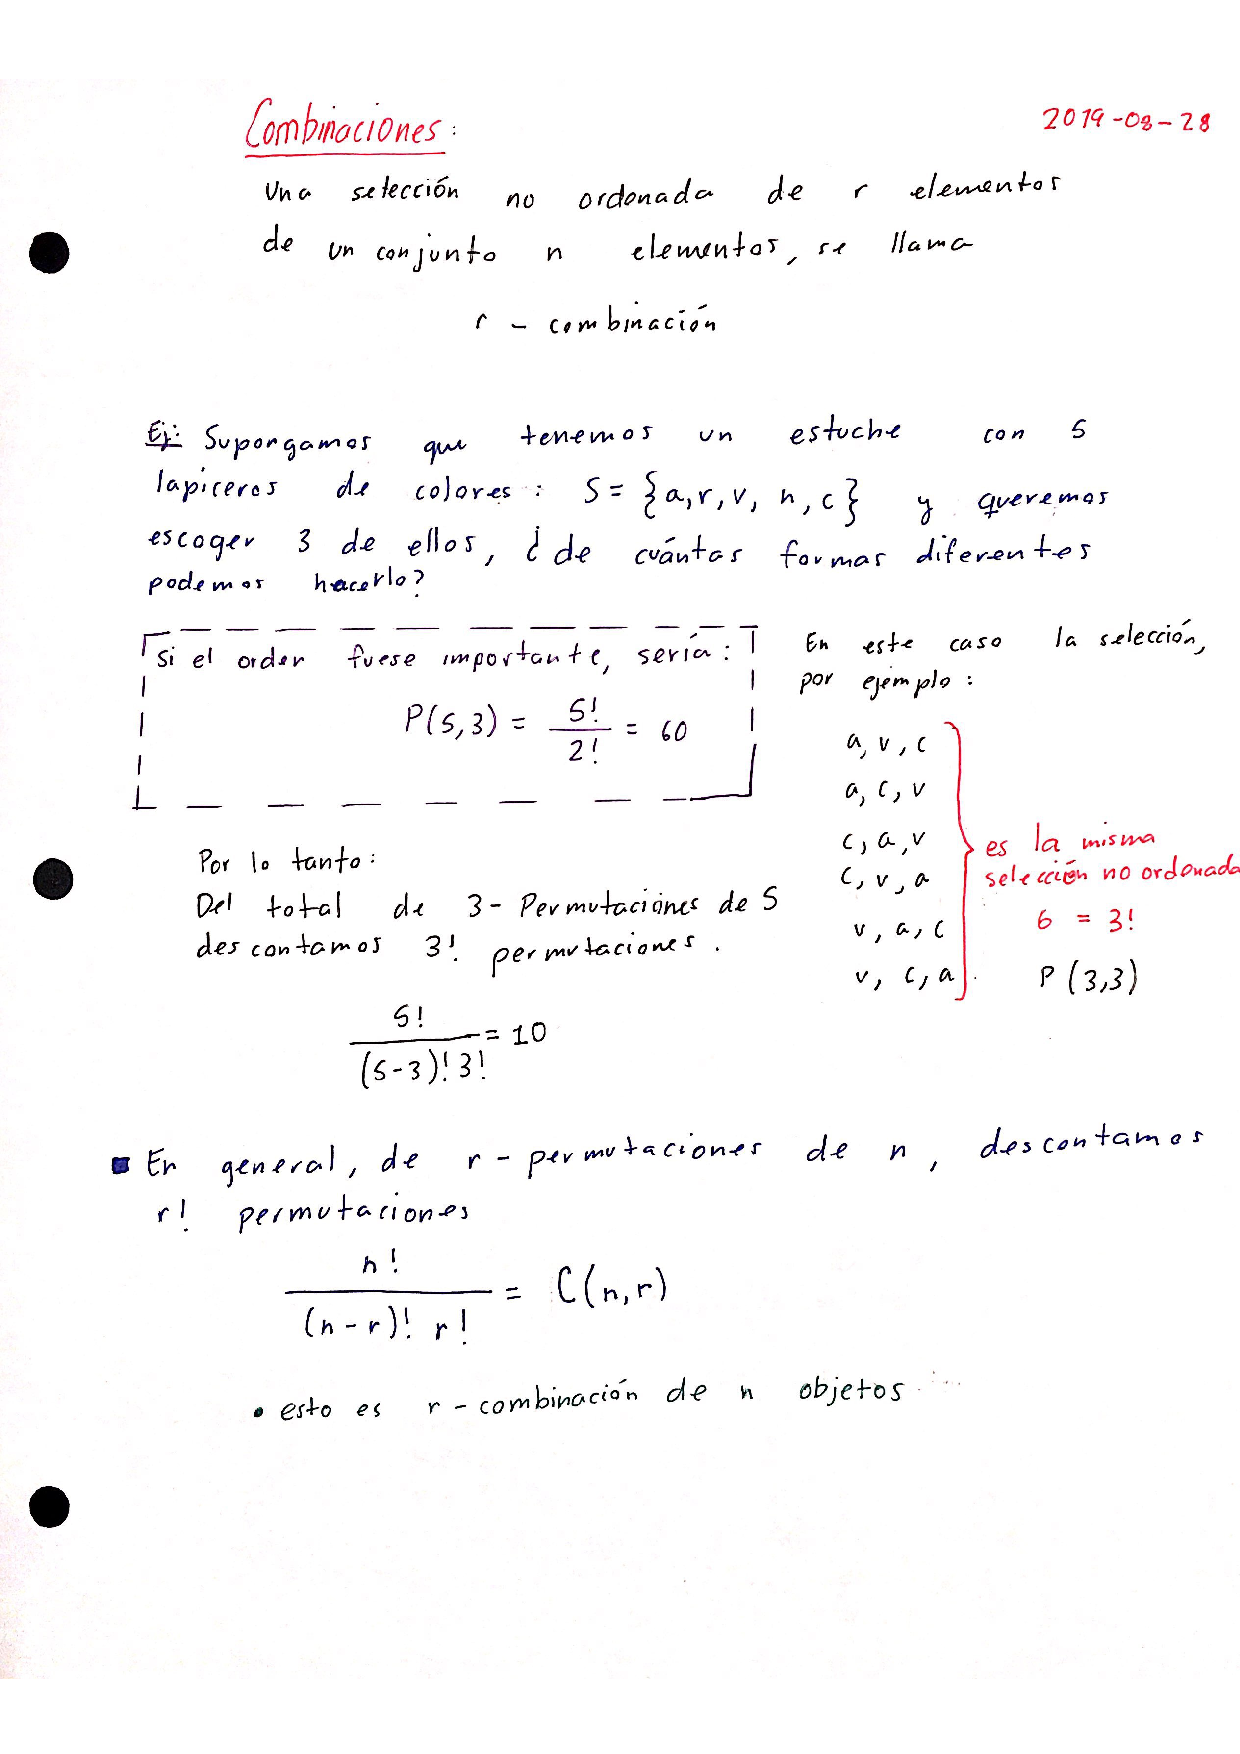
\includepdf[pages=-,pagecommand={\thispagestyle{plain}}]{Clases/2019-08-28.pdf}

\chapter{Clase del Día: 2019-09-02; Permutaciónes y combinatoria generalizada}
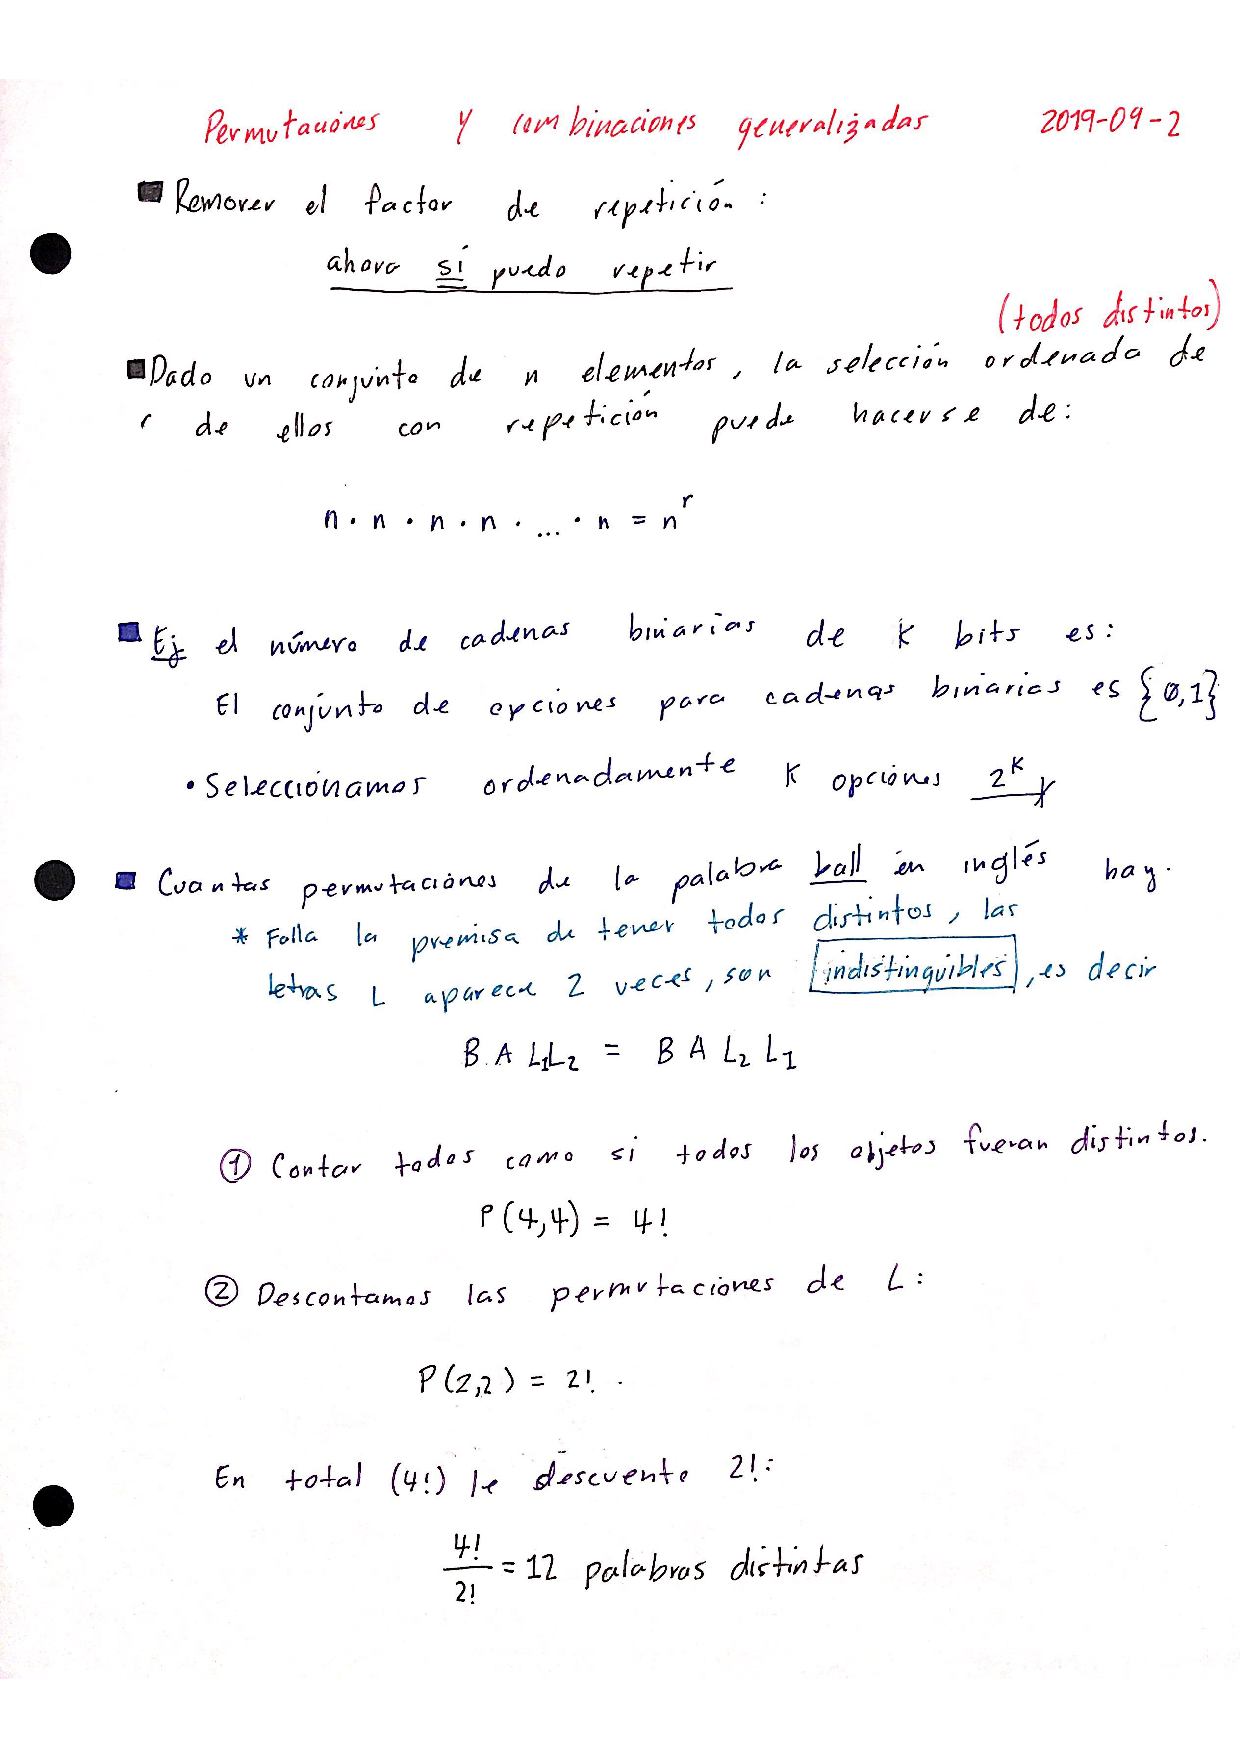
\includepdf[pages=-,pagecommand={\thispagestyle{plain}}]{Clases/2019-09-02.pdf}

\chapter{Clase del Día: 2019-09-16; Teoría de números, teorema de euclides, teorema fundamental de la aritmética, interesante: numeros primos, mcd(a,b)}
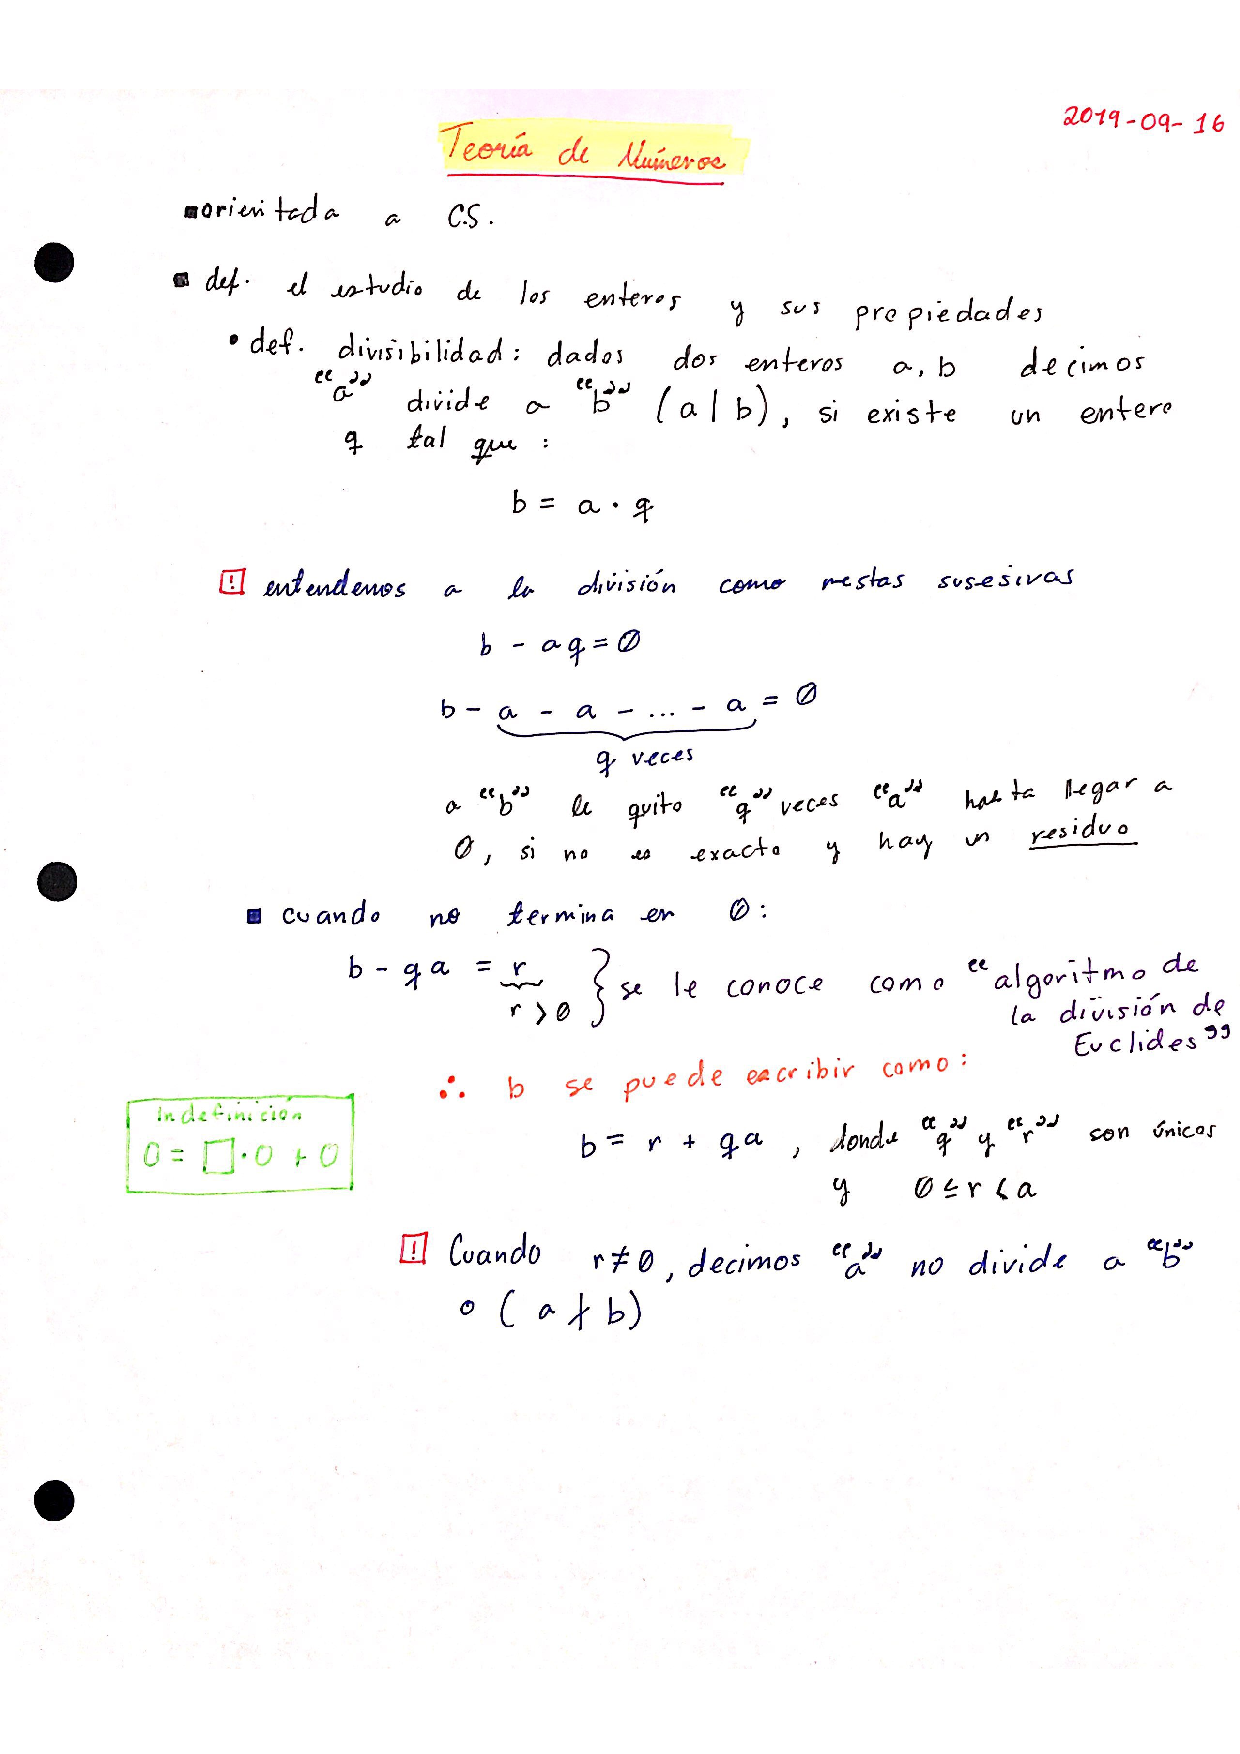
\includepdf[pages=-,pagecommand={\thispagestyle{plain}}]{Clases/2019-09-16.pdf}


\chapter{Clase del Día: 2019-09-18; Continuación, refutación del método mcd(a,b) de la mis, mínimo común multiplo (mcm(a,b)), }
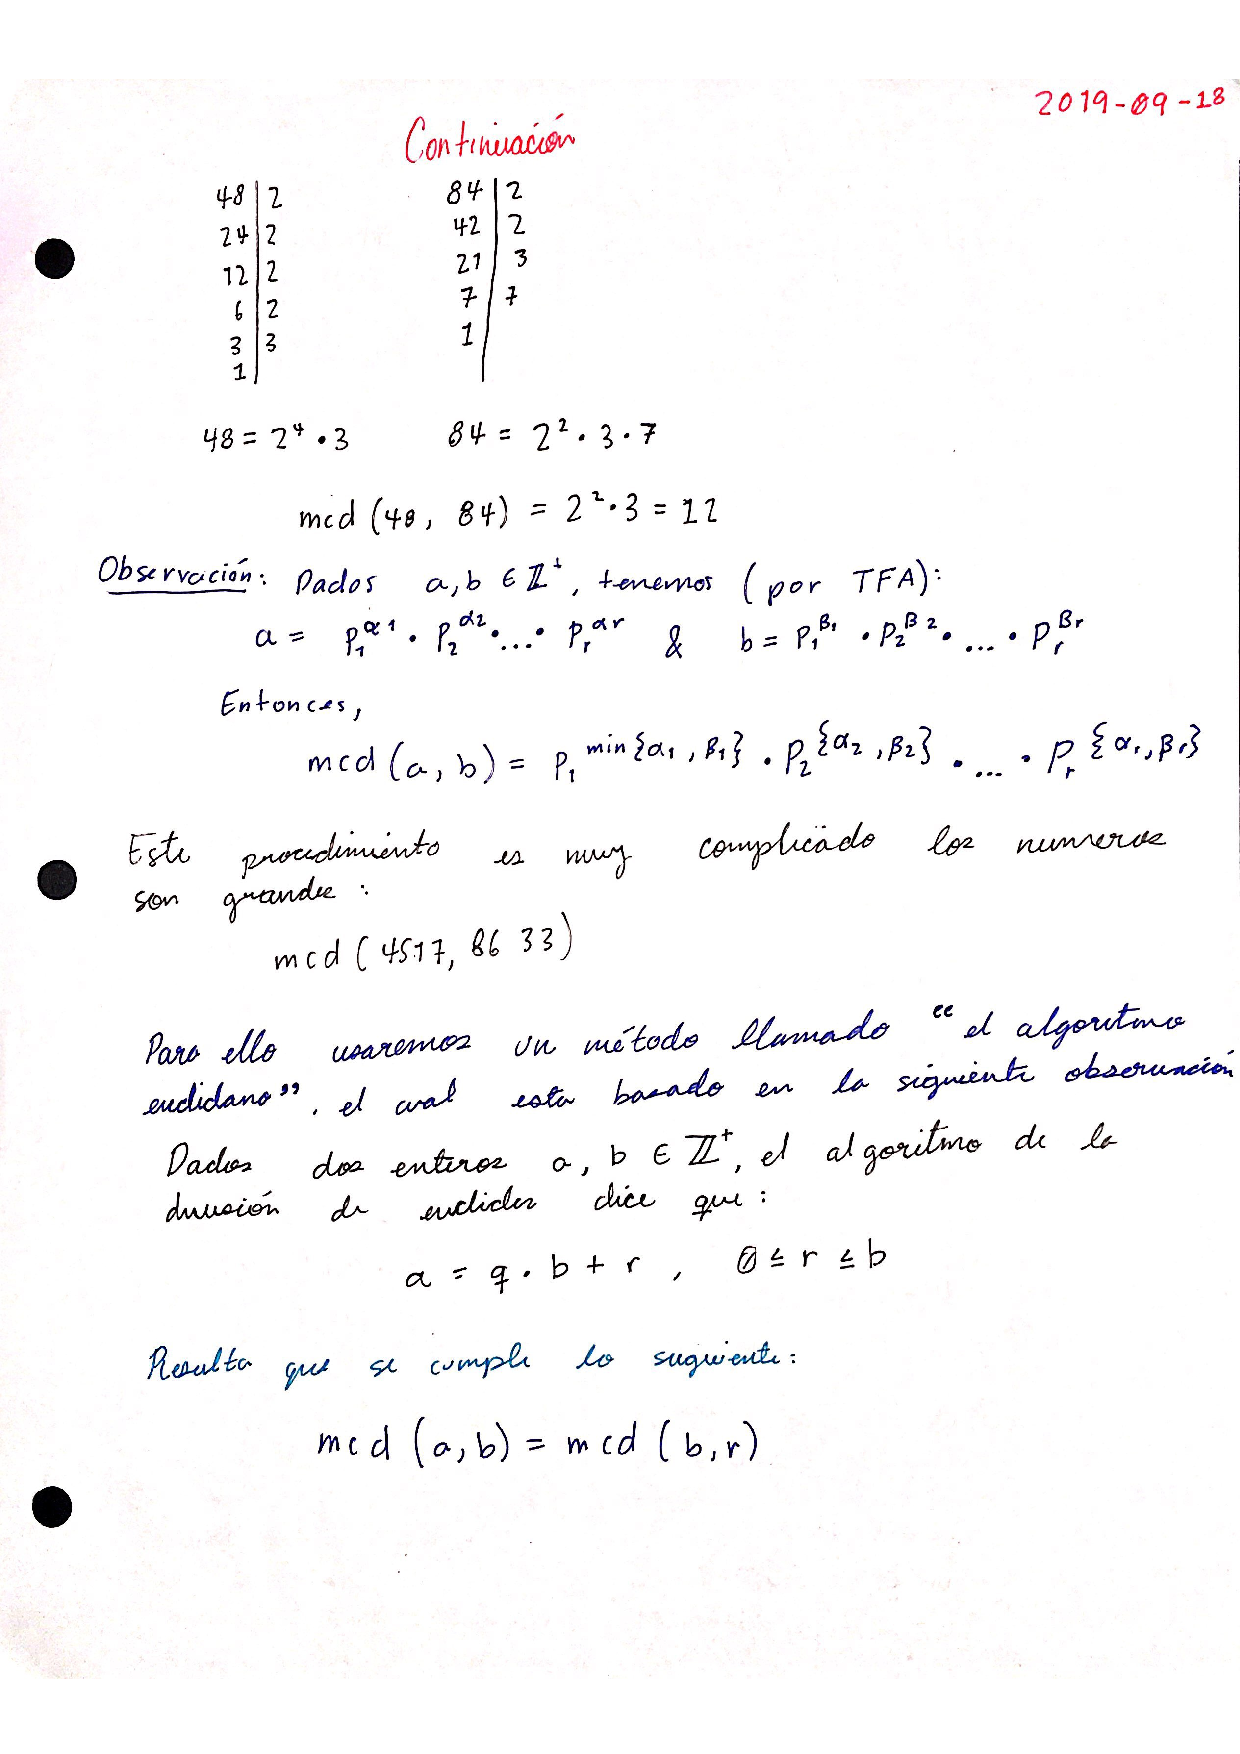
\includepdf[pages=-,pagecommand={\thispagestyle{plain}}]{Clases/2019-09-18.pdf}

\chapter{Clase del Día: 2019-09-23; Identidad de Bézout}
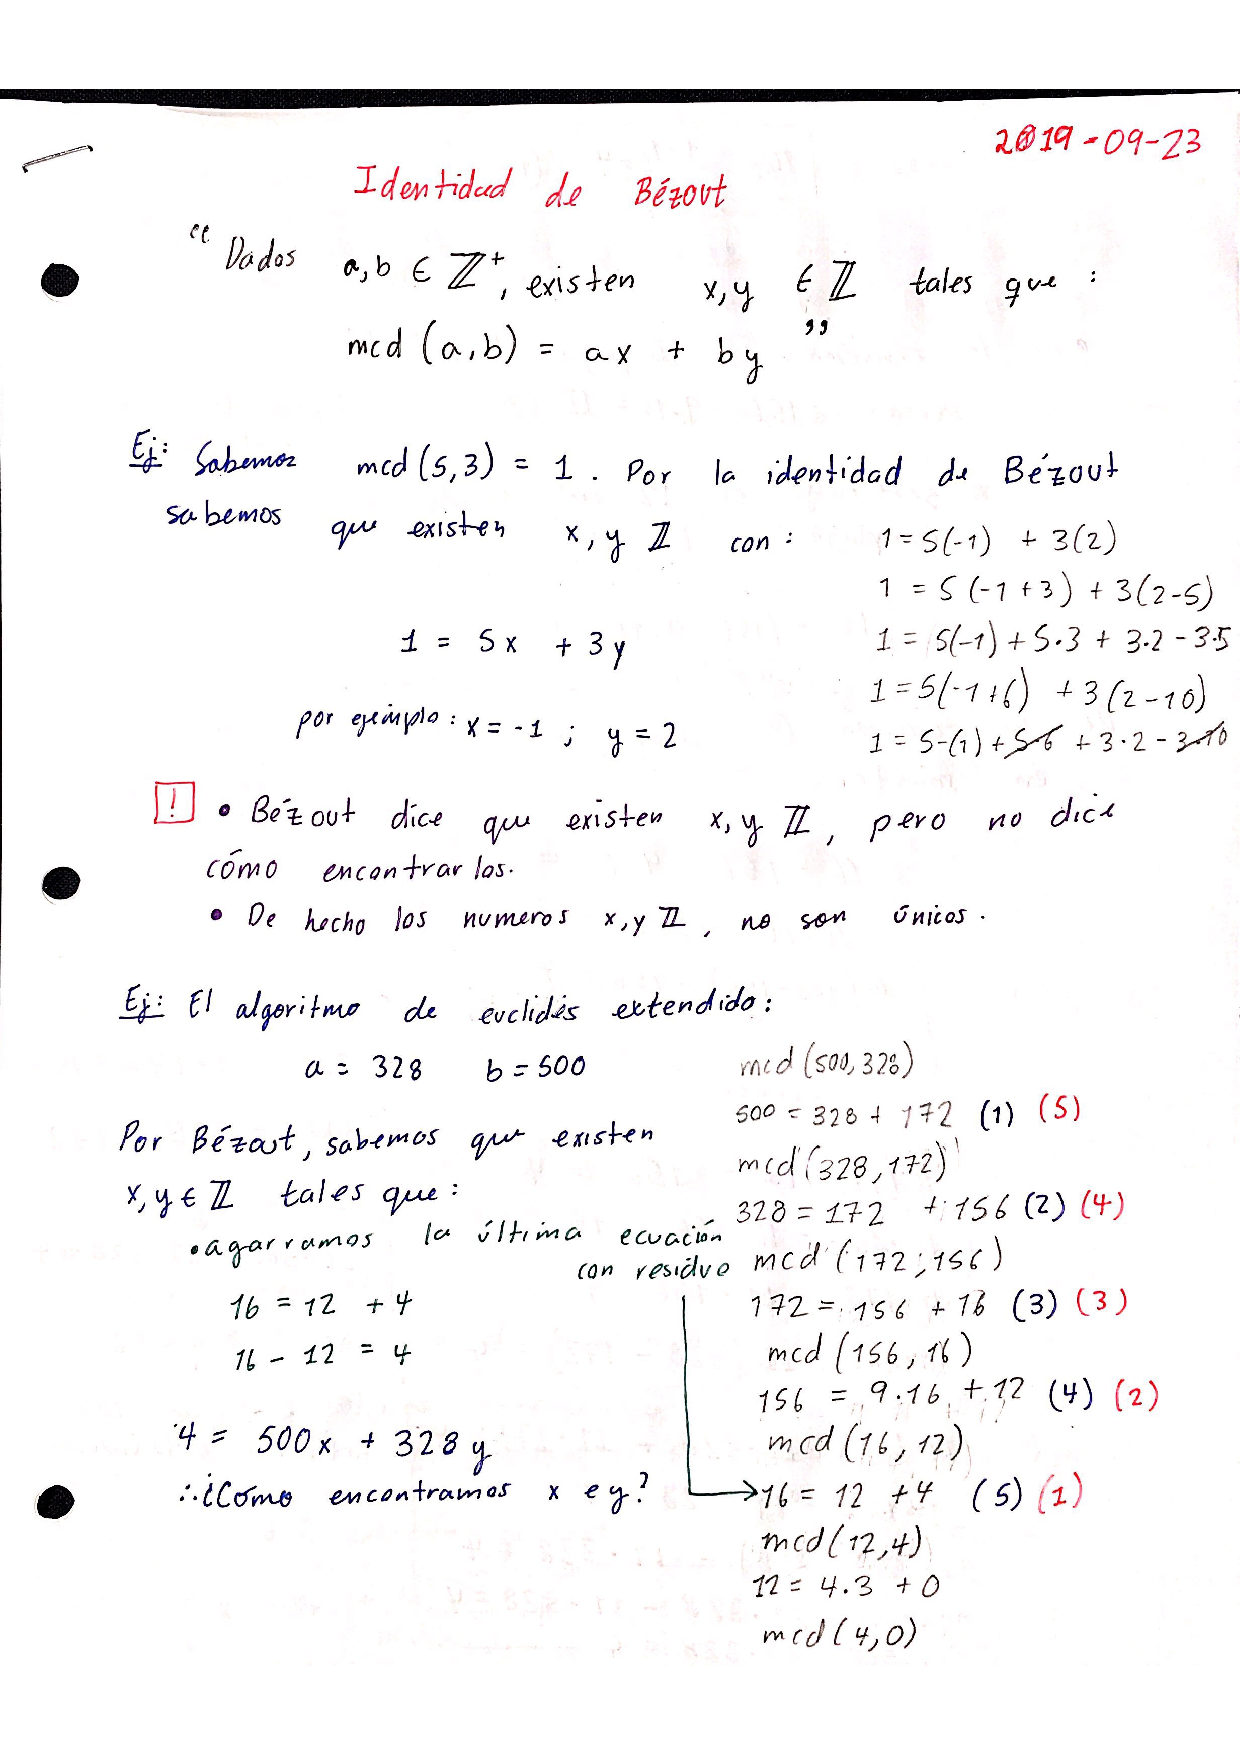
\includepdf[pages=-,pagecommand={\thispagestyle{plain}}]{Clases/2019-09-23.pdf}

\chapter{Clase del Día: 2019-09-25; Ecuación Diofantiana}
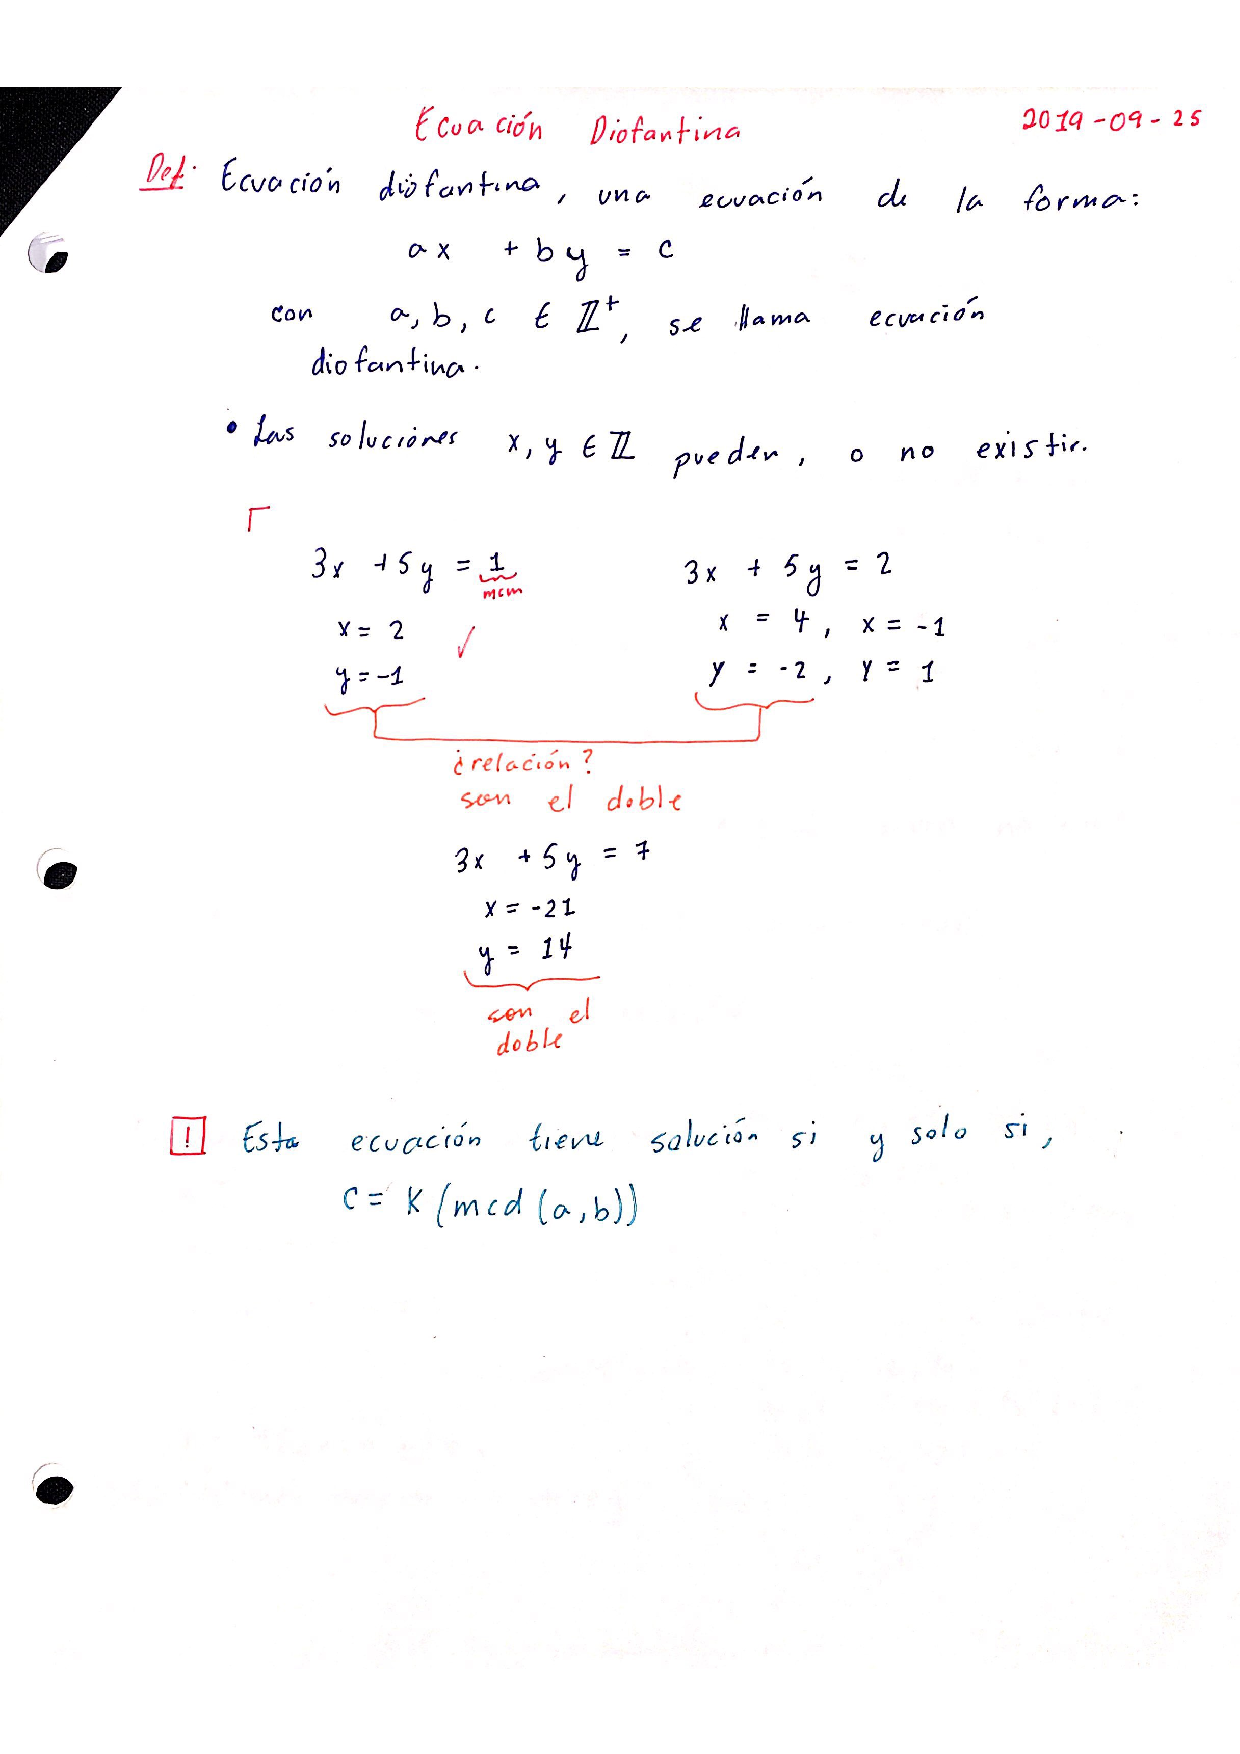
\includepdf[pages=-,pagecommand={\thispagestyle{plain}}]{Clases/2019-09-25.pdf}

\chapter{Clase del Día: 2019-09-30; Aritmética modular}
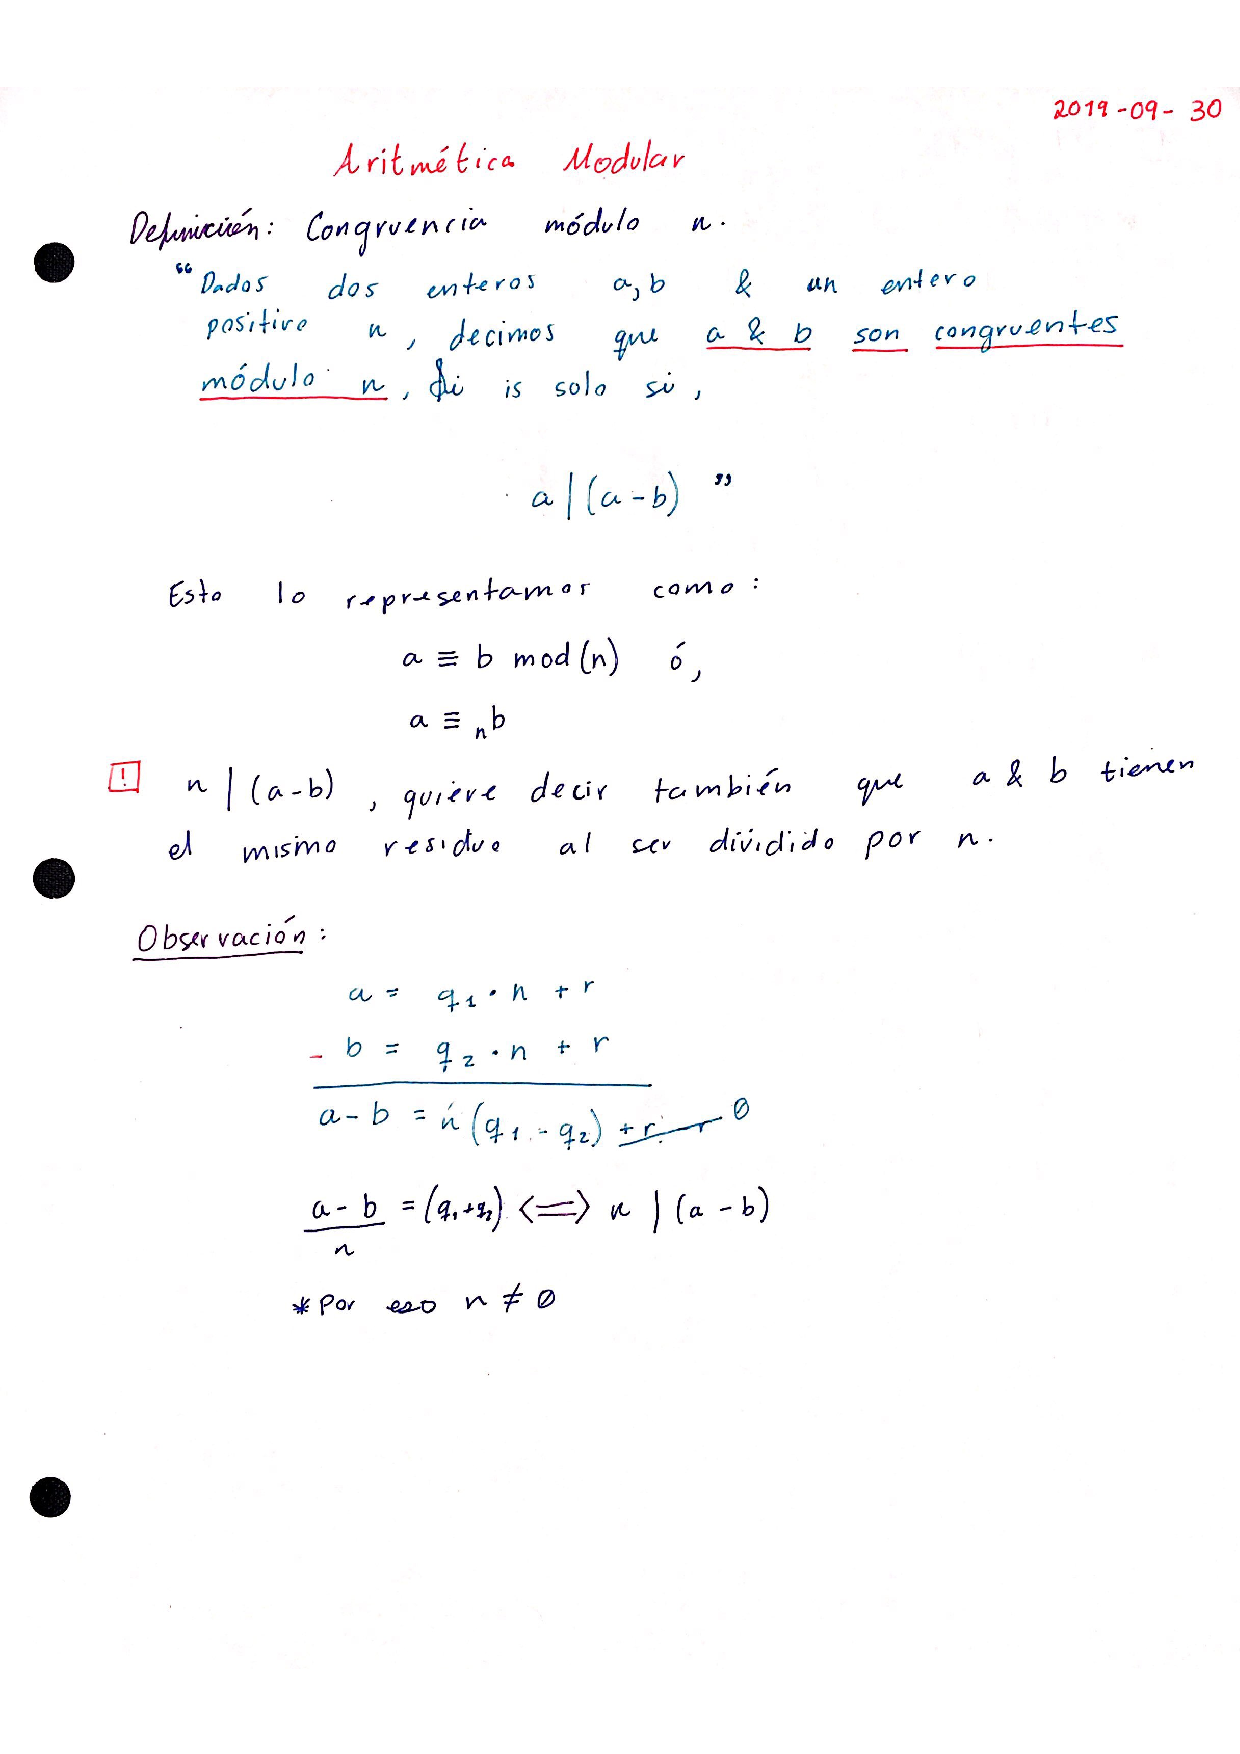
\includepdf[pages=-,pagecommand={\thispagestyle{plain}}]{Clases/2019-09-30.pdf}

\chapter{Clase del Día: 2019-10-07 ; Continuación de aritmética modular}
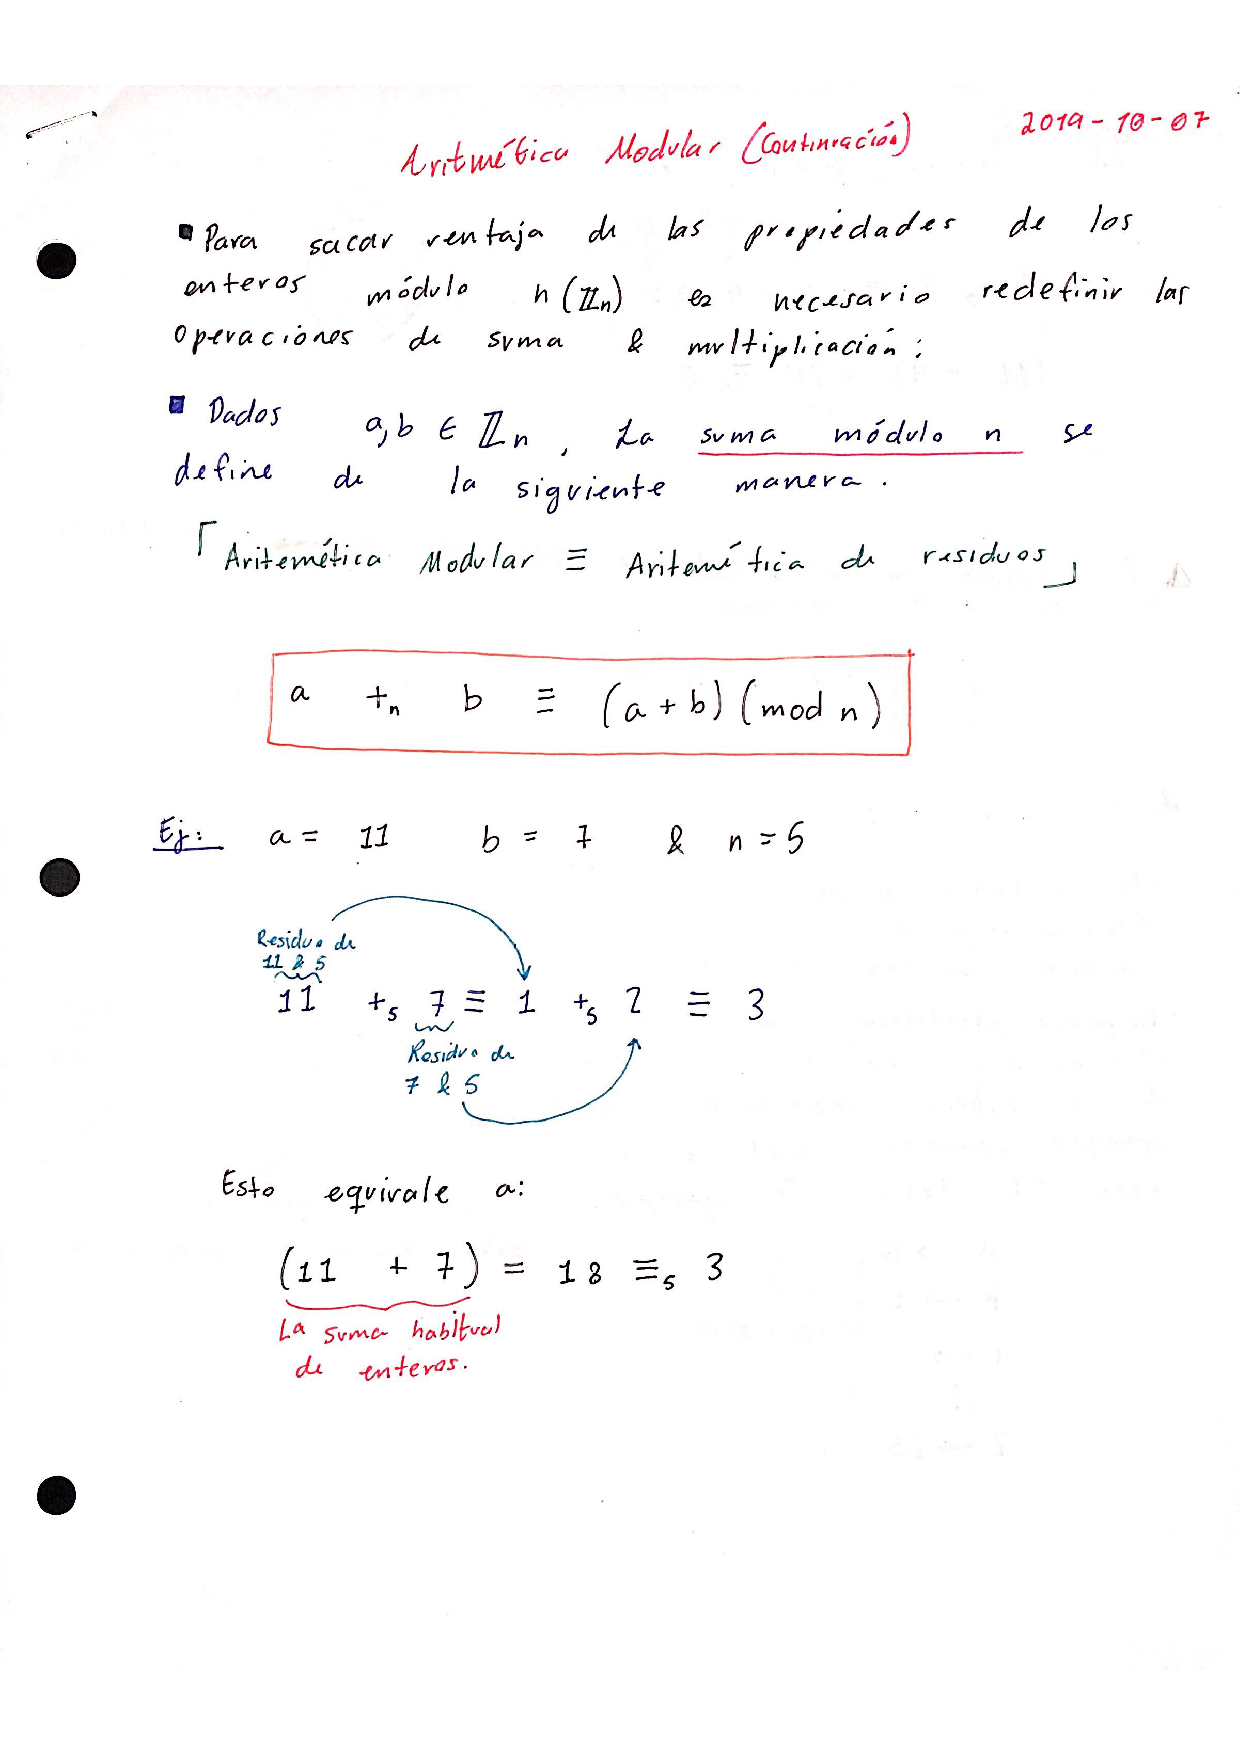
\includepdf[pages=-,pagecommand={\thispagestyle{plain}}]{Clases/2019-10-07.pdf}

\chapter{Clase del Día: 2019-10-09 ; Cálculo de inversos multiplicativos módulo $n$}
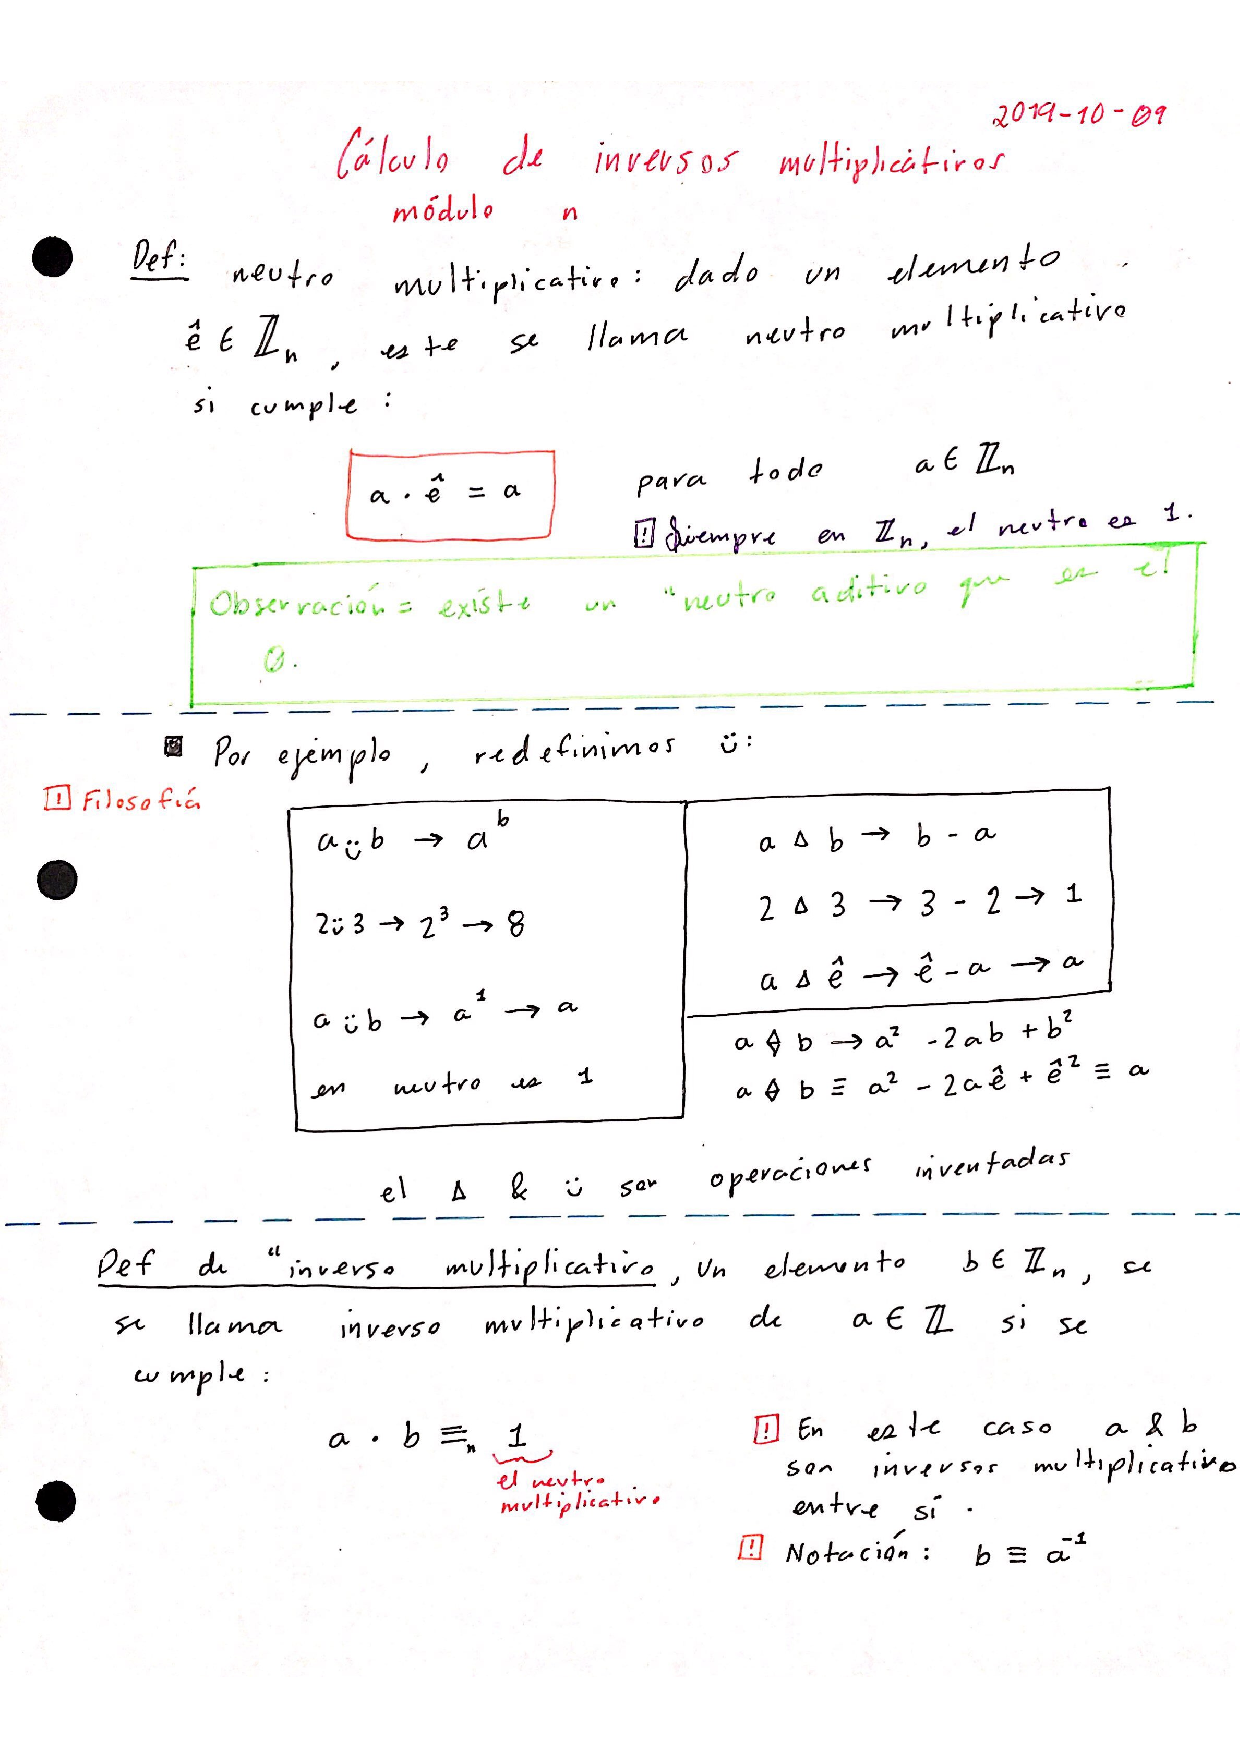
\includepdf[pages=-,pagecommand={\thispagestyle{plain}}]{Clases/2019-10-09.pdf}

\chapter{Clase del Día: 2019-10-09 ; 2019-10-16 }
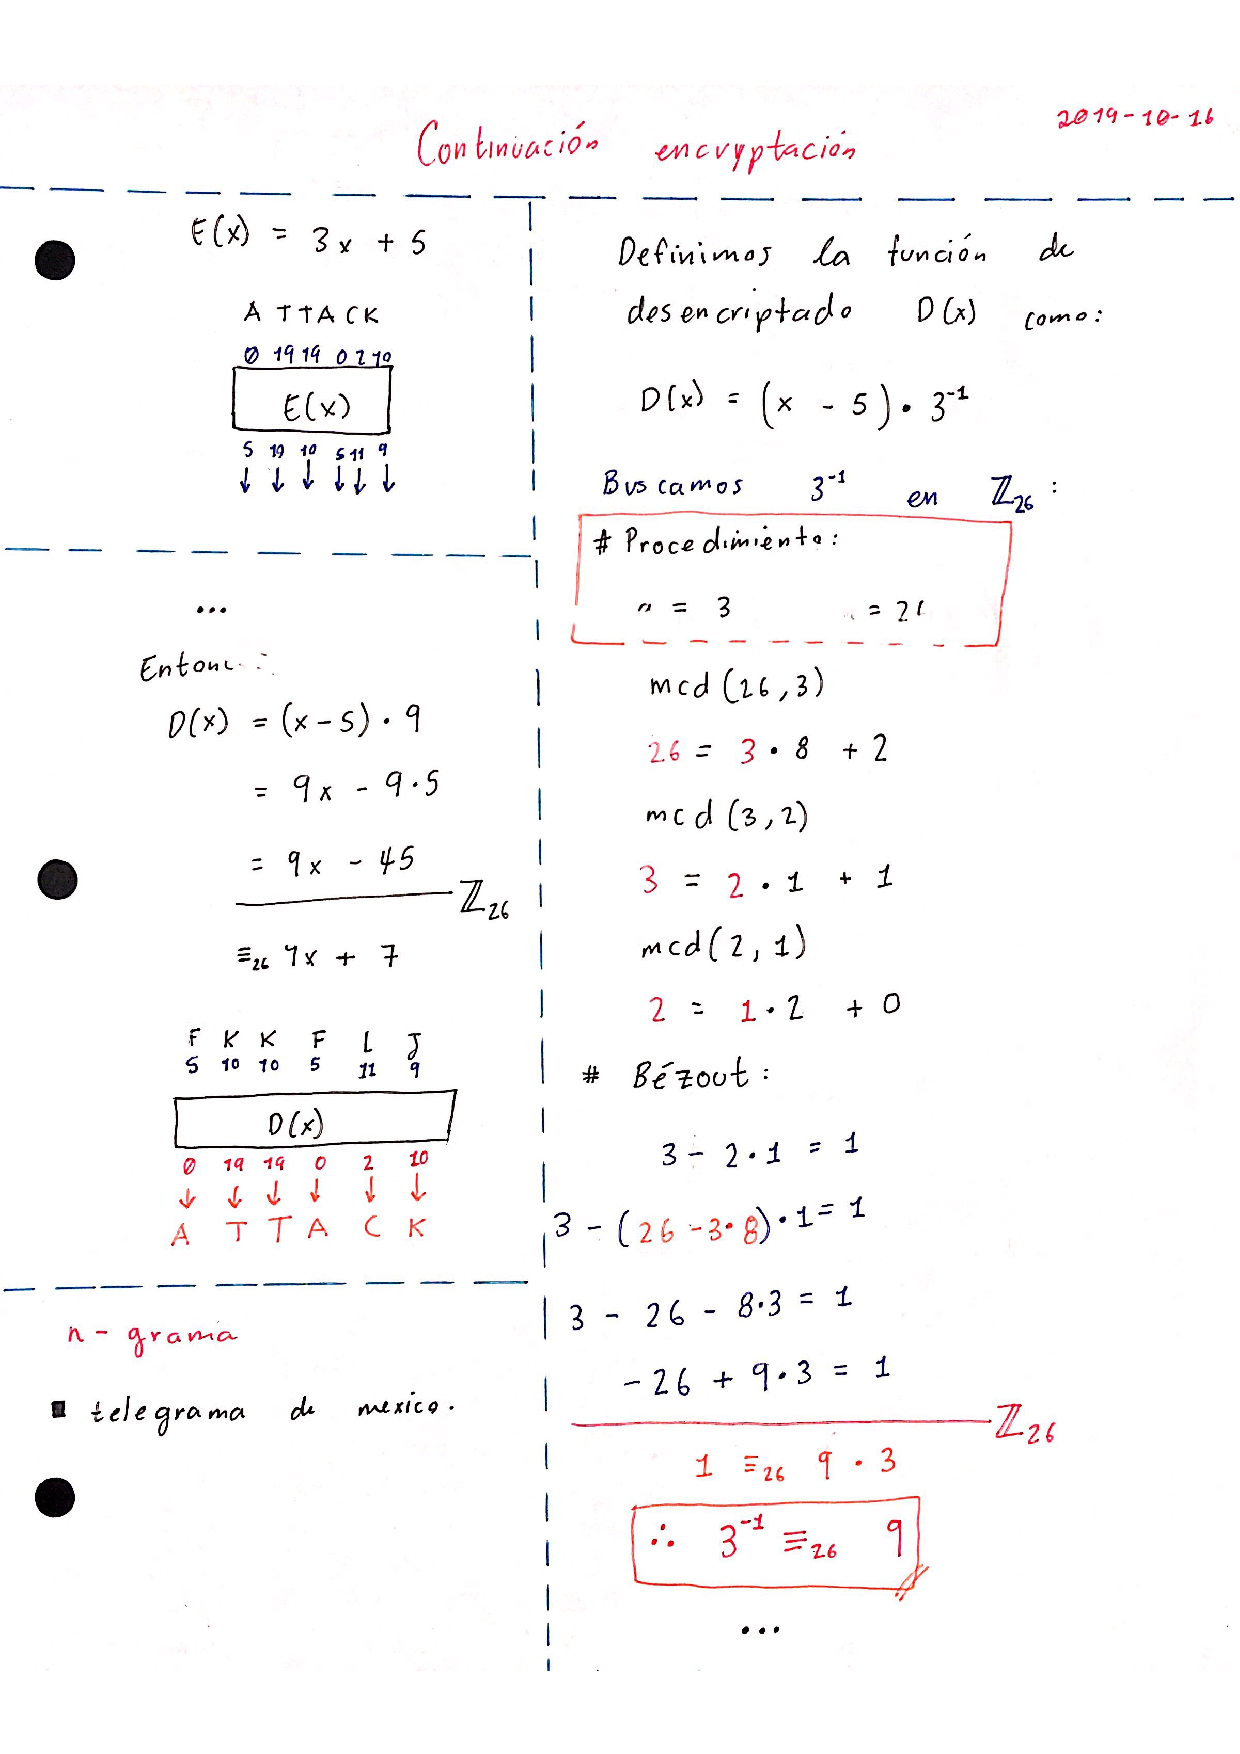
\includepdf[pages=-,pagecommand={\thispagestyle{plain}}]{Clases/2019-10-16.pdf}

\chapter{Clase del Día: 2019-10-09 ; Cálculo de inversos}
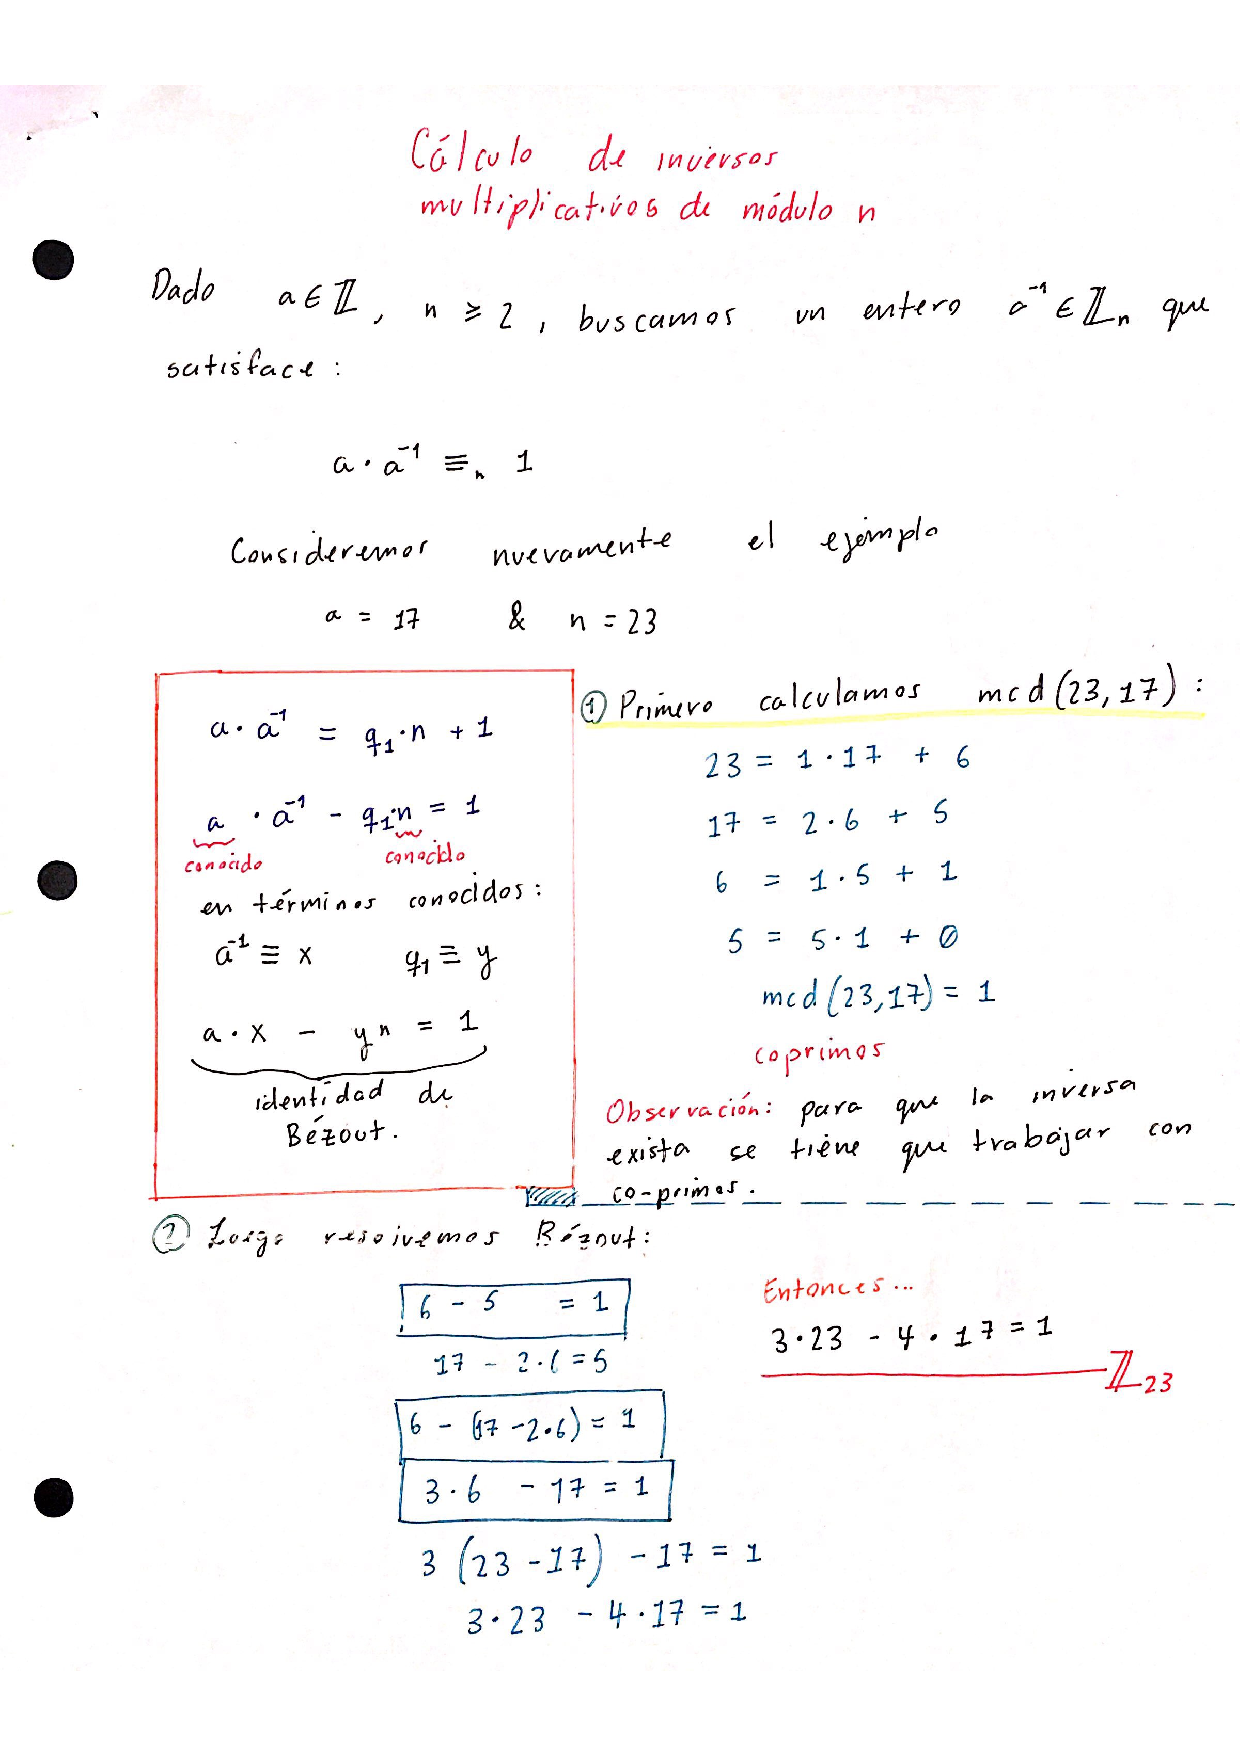
\includepdf[pages=-,pagecommand={\thispagestyle{plain}}]{Clases/CalculoDeInversos.pdf}

\chapter{Clase del día: 2019-10-30 ; Cifrado Vigenirer}
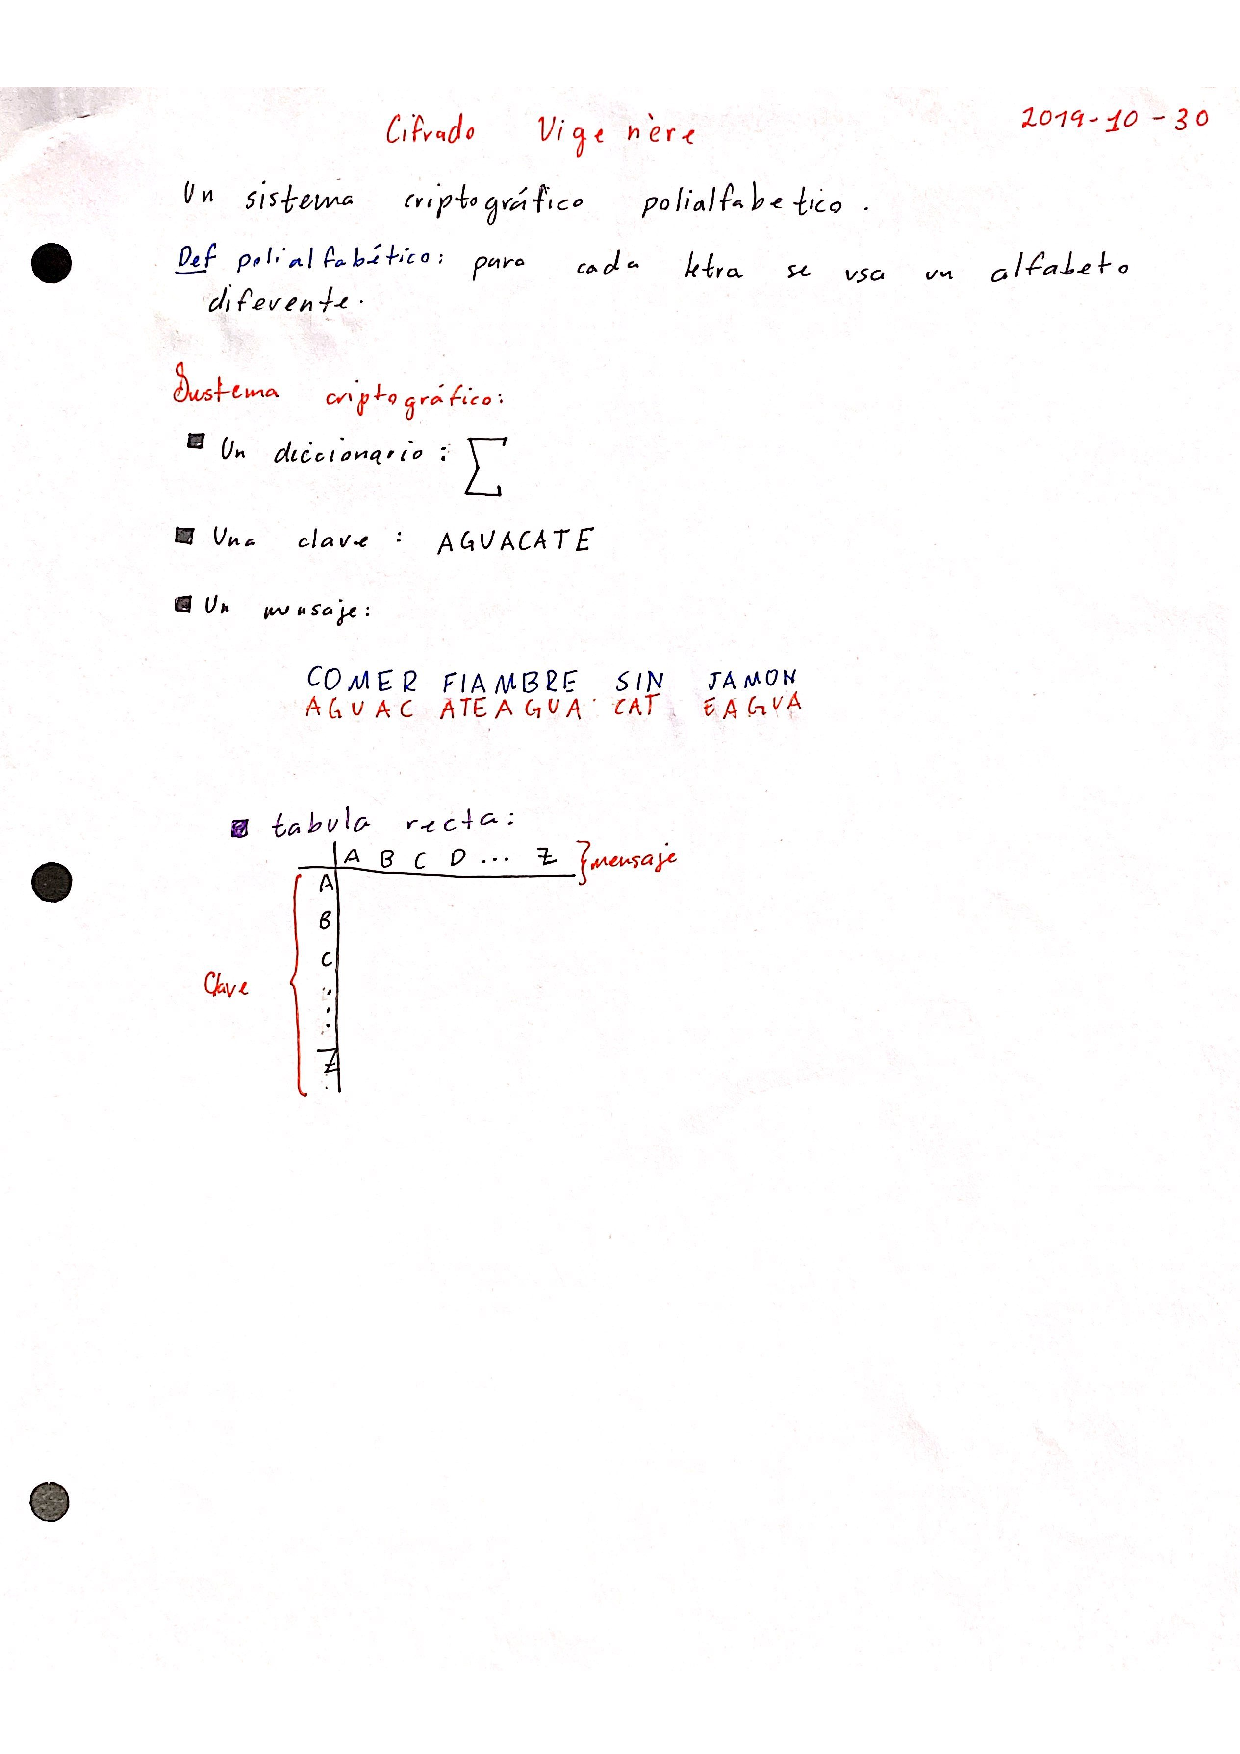
\includepdf[pages=-,pagecommand={\thispagestyle{plain}}]{Clases/2019-10-30.pdf}

\chapter{Clase del día: 2019-11-06 ; RSA, teoría}
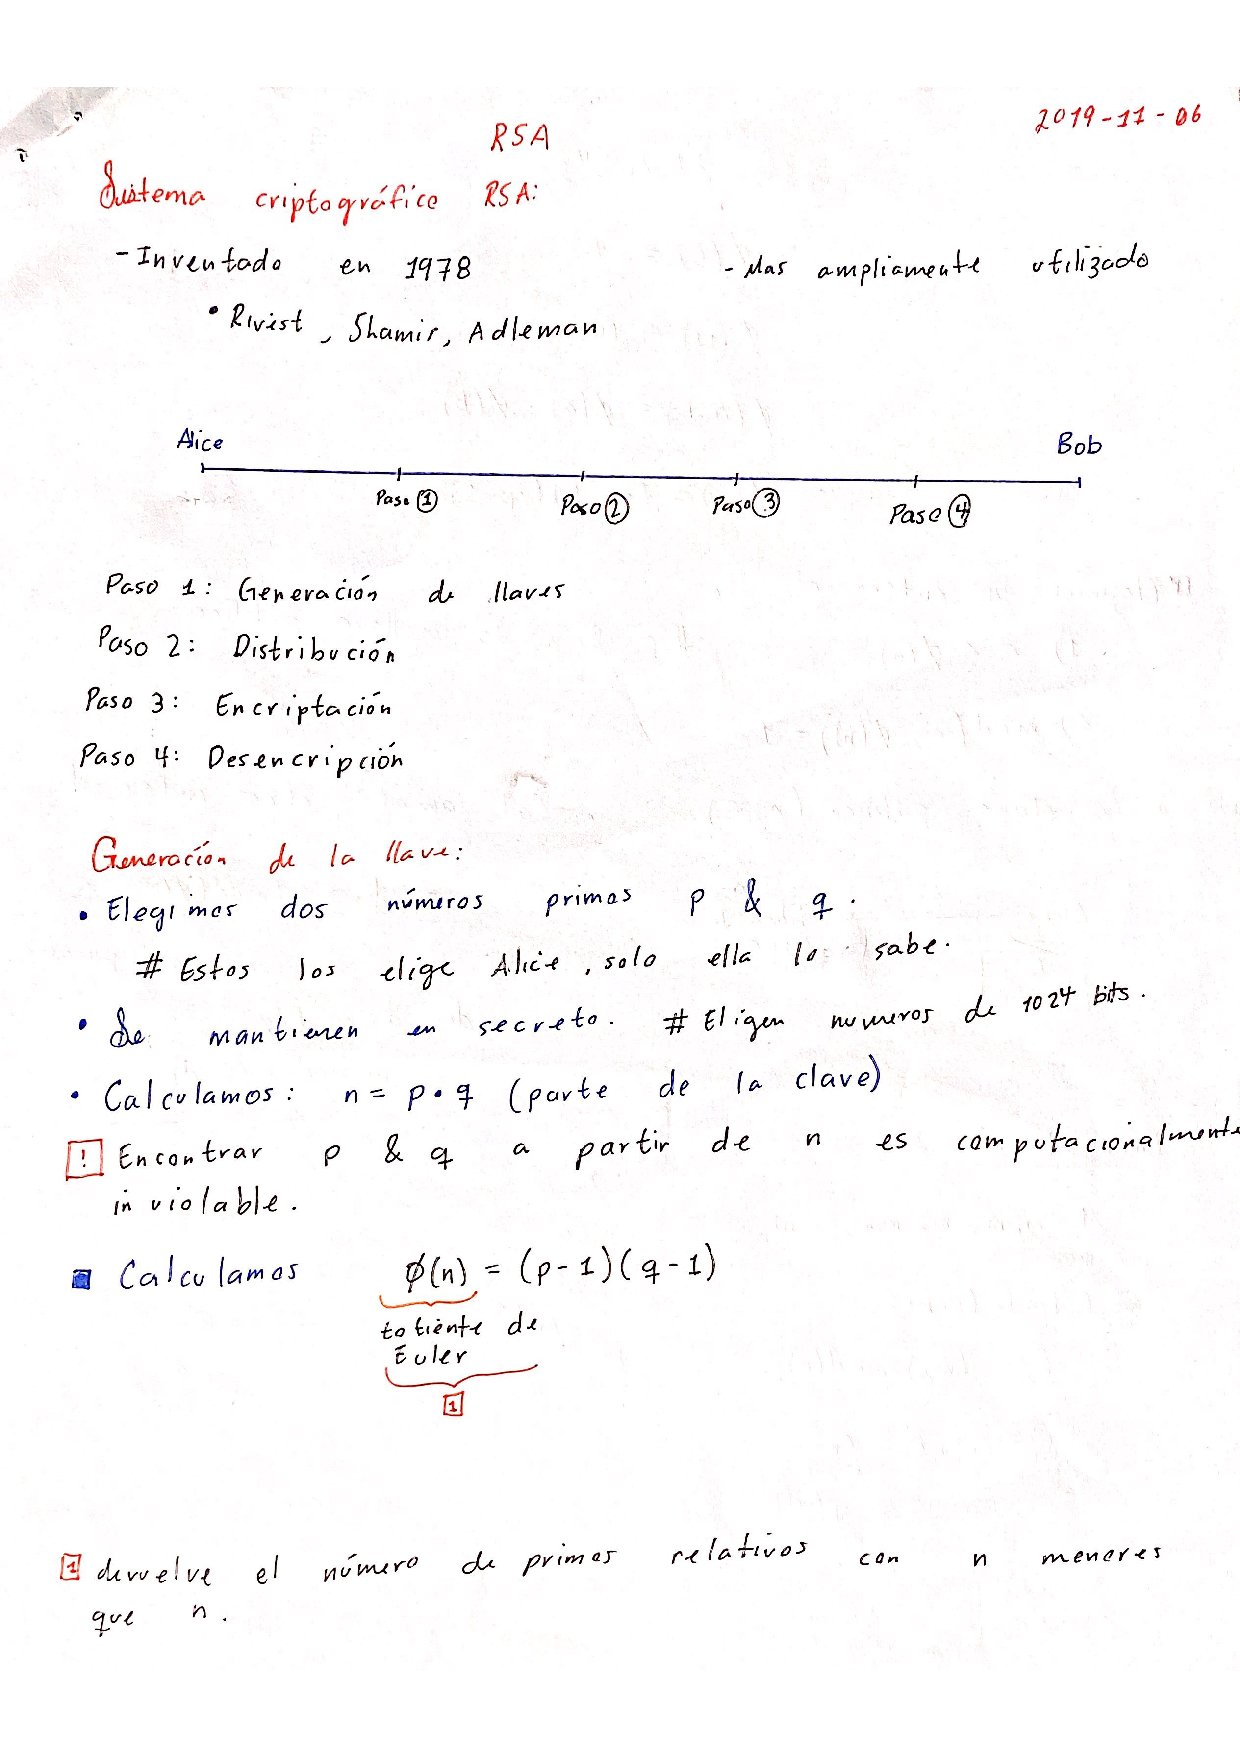
\includepdf[pages=-,pagecommand={\thispagestyle{plain}}]{Clases/2019-11-06.pdf}

\chapter{Clase del día: 2019-11-11 ; RSA, ejemplo}
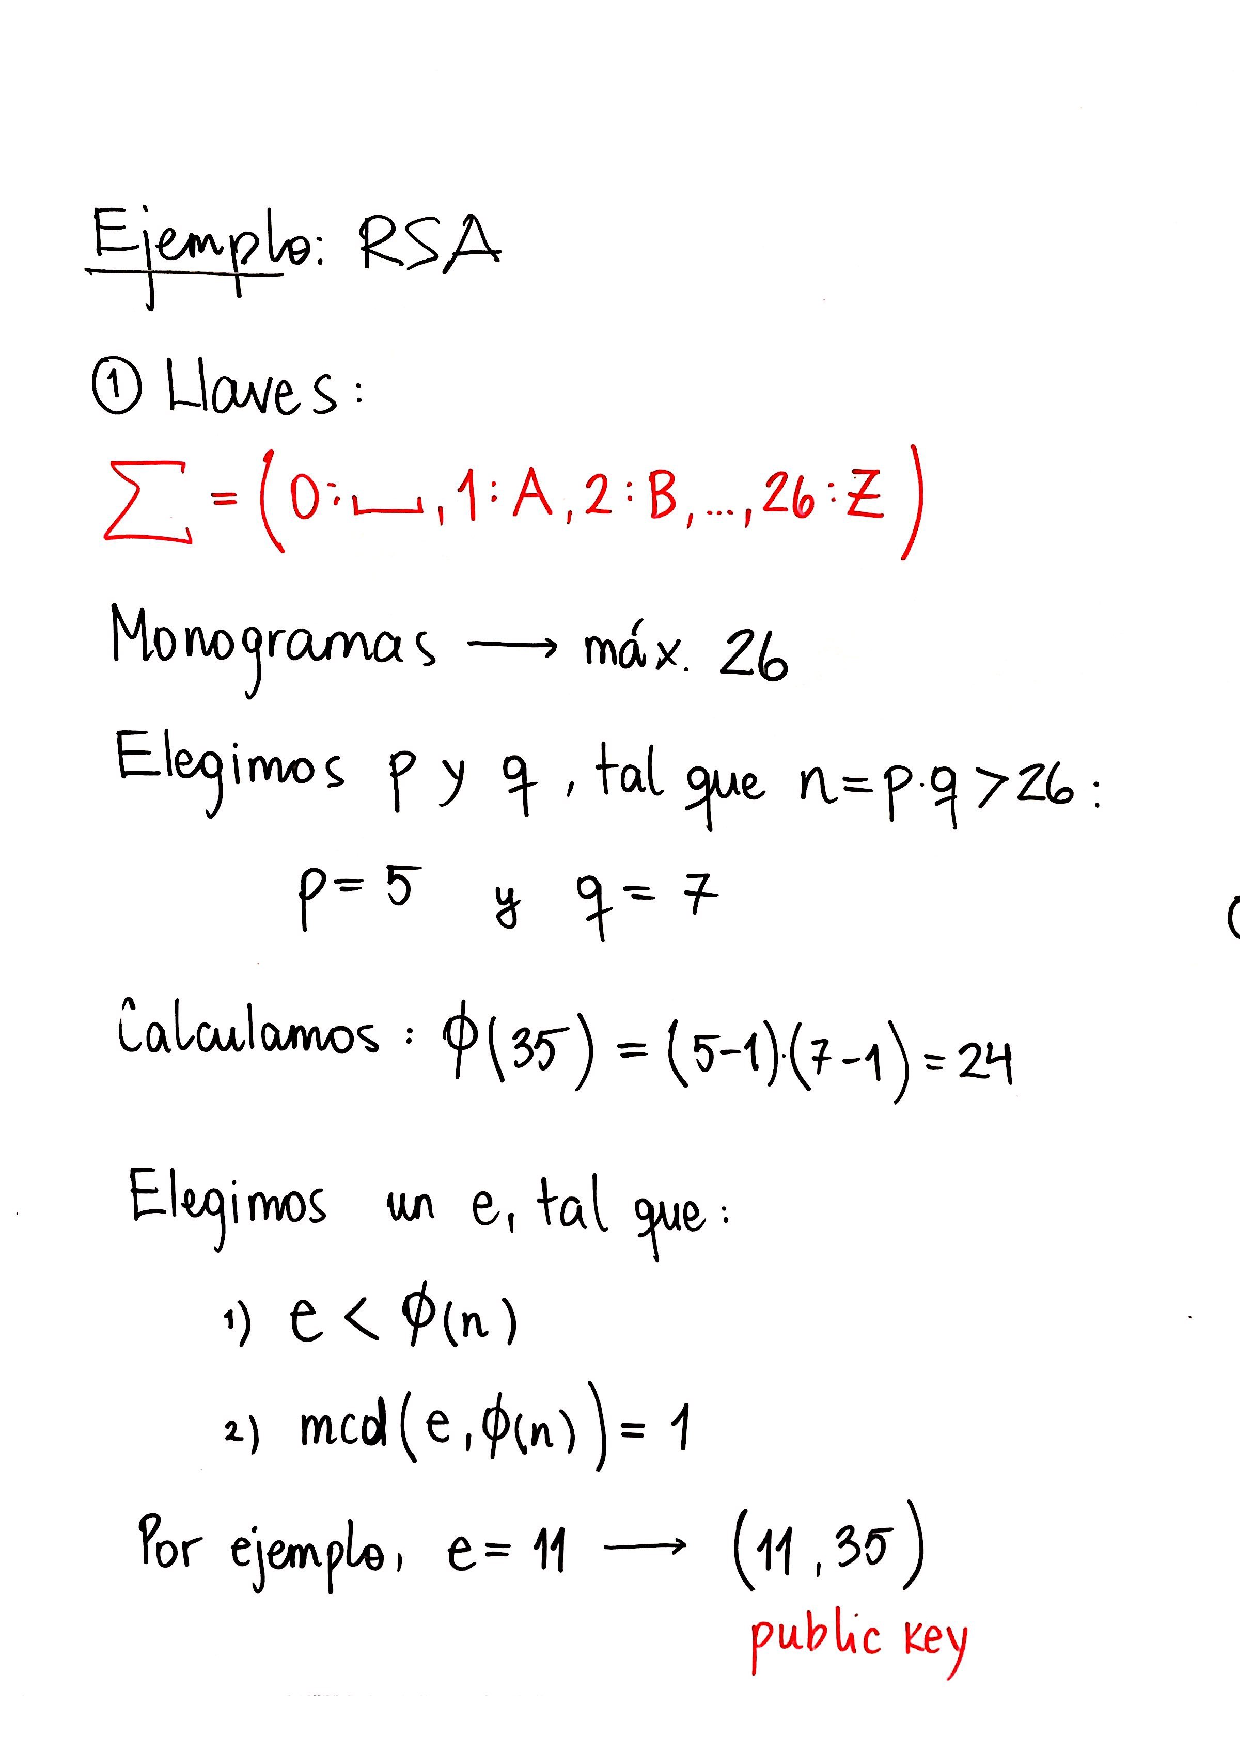
\includepdf[pages=-,pagecommand={\thispagestyle{plain}}]{Clases/2019-11-11.pdf}





\end{document}
